\section{Extended Experimental Specifications and Protocols}
\label{app:experimental_protocol}

This appendix preserves the detailed environment definitions and evaluation protocols summarized in Section~\ref{sec:experiments}.

The six environments are Tiger, Diagnosis, Bandit, Tileworld, RockSample, and Structural Inspection, and they form a progression in what the agent must decide about sensing. Tiger has a single sensor, so the only question is whether to observe again. Diagnosis and Bandit add a choice among several sensors, so the agent must also decide which observation to buy. Tileworld makes that choice spatial, with sensors that each partition a grid. RockSample and Structural Inspection interleave sensing with navigation and exploitation, so the agent must additionally move to where information is available. Four of the six (Tiger, Diagnosis, Bandit, Tileworld) follow the observe-then-commit structure of Section~\ref{sec:methodology}, in which a variable-length run of observation actions ends in a single terminal commit action and the hidden state never changes. The remaining two (RockSample and Structural Inspection) are factored observation POMDPs in the sense of Proposition~\ref{prop:factored}. Their observation, navigation, and exploitation actions interleave within an episode, which is why the paper also calls them interleaved observe-act settings.

We call Tiger, Diagnosis, and Bandit the core environments. They run at the full protocol of 1{,}000 episodes per seed across 5 random seeds ($\{42, 123, 456, 789, 1024\}$) for a total of 5{,}000 episodes. They anchor the main results table, and they are the three environments on which the near-optimal SARSOP reference of Section~\ref{sec:sarsop} is computed. Tileworld and Structural Inspection use 500 episodes per seed, and each RockSample instance uses the protocol stated in its table caption. The same agent on the same environment is also evaluated in other batteries, among them the Pareto sweep, the SARSOP and CPOMDP studies, and the shadow-price atlas, each under the episode count and seeding rule its own section states, so its usage and reward differ slightly from one battery to the next. Tiger EFE, for example, averages $4.20$ observations in Table~\ref{tab:main} and $4.32$ in Table~\ref{tab:sarsop}. Where a comparison does cross batteries, as the committed-reference column of Table~\ref{tab:budget_frontier} does, the text says so.

The rest of the protocol concerns how results are aggregated and tested. Each reported reward, success rate, and observation count is the mean over all episodes of all seeds. Pairwise statistical comparisons are seed-level Welch $t$-tests, which aggregate each seed's episodes to one mean and then test across the 5 seeds, with Holm--Bonferroni correction for multiple comparisons (Appendix~\ref{app:stats}). Bootstrap confidence intervals for the core-environment means, computed under the protocol given in the same appendix, are in the file \texttt{results\_\allowbreak bootstrap\_\allowbreak ci.csv} of the code repository. Comparison against POMCP is in Appendix~\ref{app:pomcp}. That appendix includes a scaling analysis over POMCP's simulation budget, meaning the number of simulated rollouts it runs per decision, a quantity distinct from the sensing budget $B$ of Section~\ref{sec:budget}, with wall-clock timing at 500--5{,}000 simulations per decision. Full specifications are in Appendix~\ref{app:envs}, and all environments are implemented as Gymnasium \citep{towers2024} environments, Gymnasium being a widely used Python interface for reinforcement-learning environments.

\paragraph{Tiger} \citep{kaelbling1998}. A tiger waits behind one of two doors, so the hidden state takes two values. The single observation action, listen, reports the tiger's door correctly with probability 0.85. The two commit actions open one door or the other and end the episode. A correct commit pays $+10$, an incorrect one $-100$, and each listen costs $-1$. Because there is only one sensor, Tiger poses no choice of what to observe, only whether to observe again.

\paragraph{Sequential diagnosis} (Diagnosis in tables and figures). Exactly one of $N{=}4$ hidden conditions is present, and the agent's task is to name it. There are $K{=}2$ binary tests (accuracy 0.80). Each test splits the four conditions into two groups along its own partition and reports, with that accuracy, which group contains the true condition, so the two tests together can identify any condition. There are $N$ diagnose actions, one per condition, each of which commits and ends the episode. A correct diagnosis pays $+10$, an incorrect one $-50$, and each test costs $-1$. Unlike Tiger, the agent must choose which test to run.

\paragraph{Structured bandit} (Bandit in tables and figures). One of $K{=}4$ arms is the best, and which one it is forms the hidden state. The bandit is structured in the sense that this single hidden variable, rather than an independent unknown payoff per arm, ties the arms together, so evidence about one arm is evidence about the others. Each of the $K$ inspect actions (accuracy 0.80, cost $-0.5$) targets one arm and returns a noisy yes/no signal about whether that arm is the best. Each of the $K$ pull actions commits to an arm and ends the episode. Pulling the best arm pays $+10$, and pulling any other arm pays $+1$. As in Diagnosis, the agent must choose which arm to inspect.

\paragraph{Tileworld.} Tileworld is a spatial generalization of Diagnosis. An $N{\times}N$ grid ($N{=}6$, $|S|{=}36$) hides a single target tile, and the hidden state is the cell that tile occupies. Each scan action asks a yes/no question about one binary digit of the target's row index or of its column index, and that question splits the grid in two, into the cells whose digit is 0 and the cells whose digit is 1. Three binary digits suffice to write any of the six row indices, and likewise for the six column indices. Three scans for the row digits and three for the column digits therefore give the $K{=}6$ scan actions, which together pin down the cell. Each scan alone tells the agent only which side of its own split the target lies on, and each returns its answer as a noisy binary signal (accuracy $0.80$, cost $-1$). Each of the $N^2$ commit actions declares one cell as the target's location and ends the episode (correct $+10$, incorrect $-50$). Appendix~\ref{app:envs} and Figure~\ref{fig:tw_belief} label this action collect, following the implementation. Because the belief lives on the grid itself, its evolution over an episode can be drawn directly, as shown later in Figure~\ref{fig:tw_comparison}.

\paragraph{RockSample} \citep{smith2004}. RockSample is the first environment in the suite where sensing is interleaved with movement. An $N{\times}N$ grid holds $K$ rocks at known positions, each with a hidden binary quality (good or bad), and the agent's own position is fully observable. Move actions change the agent's position. Check actions produce noisy observations of a chosen rock's quality, with an accuracy that decays with the agent's distance from that rock. Sampling collects the rock at the current position (good $+10$, bad $-10$). Exiting ends the episode from wherever the agent stands and gives $+10$. All actions cost $-0.5$. We evaluate four instances, written RS[$N$,$K$] for an $N{\times}N$ grid with $K$ rocks, namely RS[5,3], RS[7,4], RS[7,8], and RS[11,11]. Unlike the above environments, RockSample has interleaved observe-act dynamics with state transitions, the setting addressed by Proposition~\ref{prop:factored}.

This is a cost-modified variant of \citet{smith2004}'s benchmark, not the original, and it differs in six respects that a reader comparing against published RockSample numbers must know. First, every action including checks carries the $-0.5$ cost. The original charges for neither moves nor checks. It pays $+10$ for sampling a good rock, $-10$ for sampling a bad one, and $+10$ for reaching the exit, with all other moves free, so the only thing penalizing a long path there is the discount factor. Second, rock positions are fixed per instance, as in the original, but are our own choice rather than the specific maps used in the published instances. Third, returns are reported undiscounted, with episodes truncating at the $N^2{+}10K$ step cap stated in Appendix~\ref{app:envs}, whereas the original relies on its discount factor instead.

The next two differences concern the dynamics. Fourth, the exit action grants its reward from any cell rather than only at the east edge. This makes exit an unconditional outside option, that is, a fallback of known value the agent can take at any moment from wherever it stands. The POMCP analysis in Appendix~\ref{app:rocksample} turns on this fact. POMCP's search tree values each action by the mean of the returns of the simulations that pass through it (a mean backup). A guaranteed exit payoff available at every cell is the fixed alternative against which every one of those averaged estimates is measured. Fifth, the hidden rock-quality vector stays fixed when a rock is sampled. In the original, sampling a good rock turns it bad. Here, which rocks have already been sampled is tracked outside the hidden state, and the agent can recover that list from its own action history and its fully observable position. A re-sample is therefore recognized without any change to the hidden state. Re-sampling a collected rock therefore earns zero sampling reward rather than the bad-rock penalty, although the action still pays the $-0.5$ cost that every action pays. This fixity is what Proposition~\ref{prop:factored}'s application to RockSample relies on.

Sixth, the check sensor differs in both its close-range accuracy and its tail. Efficiency is the original paper's name for the sensor's reliability as a function of range. The original sensor is exact at range zero, blends toward chance as its efficiency decays with Euclidean distance, and never reaches chance at any finite range. The accuracy of our check sensor starts at $0.95$, and it is the accuracy value itself that halves with every $4$ cells of distance and is then floored at $0.5$ (\texttt{rho\_\allowbreak aif/\allowbreak environments/\allowbreak rocksample.py}). The decay meets that floor at a range of $3.7$ cells, a little short of one full halving distance because the accuracy starts at $0.95$ rather than at $1$. Since a binary observation with accuracy $0.5$ is a coin flip, our sensor is exactly uninformative beyond $3.7$ cells rather than asymptotically so.

The undiscounted, check-charging reward model is what makes sensing usage directly interpretable as a budget in Section~\ref{sec:budget}, which is why we adopt it. But it means the absolute returns reported here are not comparable to RockSample values in the literature. We use $|S|$ throughout for the number of hidden-state configurations ($2^K$ rock-quality vectors), excluding the fully observable agent position, so our $|S|{=}2{,}048$ for RS[11,11] is not the convention under which the literature quotes larger state counts for the same instance.

\paragraph{Structural inspection.} In Structural Inspection, $N$ components sit at known spatial locations on a grid, and each has a hidden binary state (nominal/faulty, prior $p_{\text{fault}}{=}0.3$) that the agent is tasked with declaring. There are $K{=}2$ non-destructive test types, visual (accuracy $0.70$, cost $-0.5$) and detailed (accuracy $0.90$, cost $-2$). The agent navigates between components, runs tests, and declares a diagnosis for one component at a time, in whatever order its own navigation takes it, so a completed episode carries one declaration per component rather than a single terminal commit. An episode ends once every component has been declared, or earlier at a step cap. A correct nominal declaration pays $+2$, a correct fault declaration pays $+5$, a missed fault costs $-50$, a false alarm costs $-5$, and each move costs $-0.5$. Neither tests nor moves change fault states, so this is a factored observation POMDP. The environment maps directly to industrial inspection, medical screening, and fault detection domains. We evaluate $N{=}8$ ($|S|{=}256$) and $N{=}16$ ($|S|{=}65{,}536$).

Two additional environments, reported in the appendices, test the EFE agent in mild-penalty and small-state-space settings and mark the boundary of the settings in which the main results apply. The two-state testbed (Appendix~\ref{app:testbed}) pairs the smallest possible hidden state with a penalty for a wrong commit that is only as large as the reward for a correct one, so that a further observation has little reward to buy. Navigation (Appendix~\ref{app:navigation}) has no separate menu of observation actions at all, since information arrives only as a side effect of moving.

\section{Extended Budget Evidence}
\label{app:extended_budget_evidence}

The following studies retain the detailed protocols, auxiliary comparisons, and robustness analyses behind Section~\ref{sec:budget_experiments}. The main text carries the primary calibration results and their principal limitations.

\subsection{Curve Collapse across Reward Scales}
\label{app:scale_details}

This subsection tests the first corollary of Proposition~\ref{prop:pi1}, that usage plotted against $w/\alpha$ is one and the same curve at every reward scale. Here $\alpha$ is the reward scale of Section~\ref{sec:pi1}. On Diagnosis and Bandit we estimate the usage curve $U_\alpha$ of Equation~\ref{eq:pi1} at reward scales $\alpha \in \{0.1, 1, 10\}$. The weight grid at scale $\alpha$ is the base grid multiplied by $\alpha$, so each grid point at one scale has a partner with the same $w/\alpha$ at the other two. The curves can be compared point by point. Figure~\ref{fig:collapse} first shows how the Diagnosis usage curves shift along the raw weight axis as rewards and costs are rescaled, then shows how dividing the weight by the same scale restores their agreement. Every matched $w/\alpha$ point coincides exactly across scales, bit-exact rather than merely within $2\cdot\mathrm{SE}$. The agreement can be exact rather than statistical because the pipeline seeds every episode's environment stream, so an agent that takes the same actions sees the same outcomes. The crossing bracket of budget $B{=}8$ in $w/\alpha$ units likewise coincides across $\alpha$ ($(0.141, 0.323]$ at every scale). We extend the check to Tiger and Tileworld-$6{\times}6$ to avoid resting the headline claim on two environments (Table~\ref{tab:collapse-breadth}).

\begin{table}[t]
\centering
\caption{Curve-collapse breadth. Fraction of matched $w/\alpha$ points across $\alpha \in \{0.1,1,10\}$ within $2\cdot\mathrm{SE}$, and whether the $B$-crossing bracket coincides across scales (in $w/\alpha$ units).}
\label{tab:collapse-breadth}
%% Numbers in this table are produced by experiments/run_price_of_information.py --mode full --only scale
\tablefontsize
\begin{tabular}{lccp{3.3cm}}
\toprule
Environment & \shortstack{Within\\$2\cdot\mathrm{SE}$} & Max spread & Bracket at $B$ \\
\midrule
\shortstack[l]{Diagnosis\\($B{=}8$)} & $100\%$ & \shortstack{$0.00$ obs.\\(bit-exact)} & $(0.141, 0.323]$ at every $\alpha$ \\
\shortstack[l]{Bandit\\($B{=}8$)} & $100\%$ & \shortstack{$0.00$ obs.\\(bit-exact)} & $(3.84, 8.76]$ at every $\alpha$ \\
\shortstack[l]{Tiger\\($B{=}4$)} & $100\%$ (trivial) & \shortstack{$0.00$ obs.\\(bit-exact)} & unbracketed ($B$ below observed $U$ at every $\alpha$) \\
\shortstack[l]{Tileworld-$6{\times}6$\\($B{=}15$)} & $100\%$ & \shortstack{$0.00$ obs.\\(bit-exact)} & $(5.80, 20.0]$ at every $\alpha$ \\
\bottomrule
\end{tabular}
\end{table}

Every environment shows bit-exact collapse, and every crossing bracket coincides across scales down to floating-point noise ($\le 10^{-15}$). This is the strongest form the check can take, and it is available only because environment streams are seeded per episode. The collapse CSVs were regenerated under the relative comparison tolerance of Section~\ref{sec:pi1} and are byte-identical to those produced under the earlier absolute tolerance, which did not bind at any swept point. Tiger passes trivially. Instrumental listening already saturates usage (constant $4.37$ observations at every grid point) across the entire $w/\alpha \in [0,20]$ range tested, so the budget formulation has no usable dial in this window. Proposition~\ref{prop:pi1} guarantees collapse of whatever curve there is, not that every environment has an informative curve to collapse.

\subsection{Proposition~\ref{prop:nearopt} Onset on Positive-Threshold Two-State Instances}
\label{sec:prop2exp}

This subsection checks that the closed-form onset threshold $w_{\mathrm{thresh}}$ of Proposition~\ref{prop:nearopt}, the weight above which observing first switches on, is where the measured usage staircase takes its first upward step, as Corollary~\ref{cor:pi4} predicts. The check needs instances whose threshold is positive. Standard Tiger and Testbed parameters yield negative $w_{\mathrm{thresh}}$, so any $w \ge 0$ observes. The check of Corollary~\ref{cor:pi4} is vacuous there. We therefore construct two positive-threshold Testbed instances. Each is the two-state Testbed environment of Appendix~\ref{app:testbed} (the \texttt{InfoSeekingEnv} class of the implementation), whose standard parameters are tabulated in Appendix~\ref{app:envs}. At each step the agent chooses between committing at once and paying cost $c$ for one more observation of accuracy $p$. The two instances differ from the standard Testbed only in a costlier, less accurate observation ($p \in \{0.60, 0.58\}$, $c{=}0.3$, $R_\pm = \pm 1$, where $R_\pm$ are the correct-commit reward and the incorrect-commit penalty). One point of notation before the numbers. The $\alpha$ of Proposition~\ref{prop:nearopt} is its reward asymmetry ratio $|R^-|/R^+$, a different quantity from the reward scale that Section~\ref{sec:collapse} writes with the same letter. With symmetric rewards these instances have $\alpha{=}1$, the boundary of the proposition's strict asymmetry hypothesis, but the threshold formula itself does not require that hypothesis. Their closed-form thresholds are $w_{\mathrm{thresh}} \approx 3.44$ and $7.55$ in the implementation's bit units, the convention the swept weight grid uses, equivalently $4.97$ and $10.89$ nats. A refined weight grid around the threshold shows $U{=}0$ at and below $w_{\mathrm{thresh}}$, with onset in $(w_{\mathrm{thresh}}, 1.03\cdot w_{\mathrm{thresh}}]$ on both environments (upper relative error $3\%$, Figure~\ref{fig:prop2}), matching Corollary~\ref{cor:pi4}. In words, the measured onset never falls below the closed-form threshold. The upper endpoint of the onset bracket sits within three percent of the threshold, three percent being the spacing of the first refined grid point above it, so the bracket is one grid step wide. Negative-threshold sanity checks on standard Testbed and Tiger remain consistent ($U(0) > 0$ when $w_{\mathrm{thresh}} < 0$).

\begin{figure}[tbp]
\centering
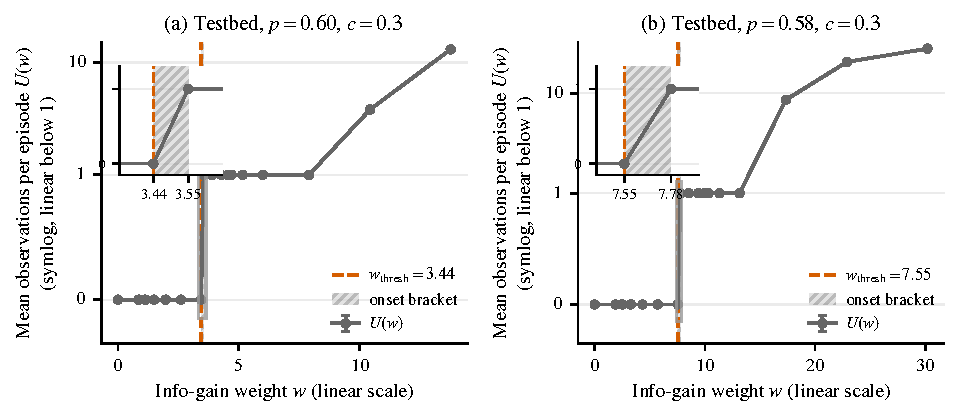
\includegraphics[width=\textwidth]{figures/price_prop2_jumps.pdf}
\caption{Onset of observing on positive-threshold testbeds. The vermillion dashed vertical line marks the $H{=}1$ closed-form threshold (Proposition~\ref{prop:nearopt}) and the hatched gray band is the empirical onset bracket after grid refinement, magnified in the zoom row beneath each main panel, with the shaded strip on the main panel marking exactly the region the zoom row below it shows.}
\label{fig:prop2}
\Description{Two columns, each with a main panel above and a smaller zoom panel below. Each main panel plots mean observations versus the weight w, on a vertical axis that is linear from zero to one and logarithmic above one, showing a gray solid curve with round markers that sits at zero, steps up to one just past a vermillion dashed vertical threshold line, plateaus at one, and then climbs at large weights to about 13 in the left column and about 28 in the right column. A light gray shaded strip on the main panel marks the narrow region around the threshold that the zoom panel beneath it magnifies. Each zoom panel repeats the same curve over just that narrow region, with the threshold line at its left edge and the hatched onset band extending to its right edge, and its own axis ticks giving the threshold and bracket-end values exactly, 3.44 and 3.55 on the left, 7.55 and 7.78 on the right.}
\end{figure}

\subsection{Multi-Seed Online Dual Control under Reward Rescale}
\label{app:dual_details}

Section~\ref{sec:pi5} argued that an offline bracket is valid only at the reward scale it was solved at, so a deployed controller must re-adapt online after an unannounced rescale, and it left the speed of that re-adaptation to be measured. This subsection measures it across controller seeds and asks whether resetting the step-size clock after a detected shift makes it faster. The step-size clock is the decay clock of Section~\ref{sec:pi5}. The setting is Diagnosis with target $B{=}8$, learning rate $\eta_0{=}0.05$, decay $\delta{=}0.02$, and a $\times 10$ reward-and-cost rescale at episode~$200$ of a $400$-episode run, and we sweep $10$ independent controller seeds for each of two variants. The decay-only variant runs the update of Equation~\ref{eq:dual_update} with its step decaying from the first episode and never intervenes. The reset-on-shift variant runs the same update and adds the change-detection heuristic of Section~\ref{sec:pi5}. It watches a rolling window of recent per-episode usage (window~$20$), and once the step has decayed below half its initial value it declares a shift when the mean usage over that window departs from $B$ by more than a threshold. That threshold is the larger of $k$ standard errors of the window mean ($k{=}3$) and an absolute floor of $0.5$ observations, so a departure smaller than $0.5$ observations never counts as a shift however small the window's standard error happens to be. A declared shift restarts the step-size clock, so the step is large again.

Re-adaptation time is measured on a rolling mean of usage that, at each post-rescale episode, averages per-episode usage over the previous $20$ episodes and is computed from post-rescale episodes only. Re-adaptation time is the number of episodes after the rescale until that rolling mean stays within $\pm 1$ of $B$ for $20$ consecutive episodes. Restricting the window to post-rescale episodes matters. A window allowed to straddle the rescale point reports a spuriously fast recovery by mixing in already-converged pre-rescale usage (\texttt{experiments/\allowbreak run\_\allowbreak price\_\allowbreak of\_\allowbreak information.py:\allowbreak readaptation\_\allowbreak episodes}).

Resetting the step-size clock re-adapts roughly $3\times$ faster than decay alone. The comparison of record uses one estimand for every seed, the restricted recovery time $\min(T, 180)$, where $T$ is the post-rescale-only recovery time and $180$ is the last index at which the $20$-episode hold can still be checked inside the $200$ post-rescale episodes, with a seed that never completes the hold scored at $180$. On that estimand decay-only averages $157.3$ episodes and reset-on-shift $51.2$. Because the two variants share their ten controller seeds, the paired difference is $106.1$ episodes with a Student-$t$ $95\%$ interval of $[96.8, 115.4]$. Every one of the ten paired differences is positive, the smallest being $89$ (\texttt{results\_\allowbreak price\_\allowbreak dual\_\allowbreak multiseed\_\allowbreak metrics.csv}, column \texttt{readapt\_\allowbreak restricted}, and the summary JSON's \texttt{dual\_\allowbreak ms\_\allowbreak readapt\_\allowbreak restricted} block). For descriptive context, we also report mean recovery times among the seeds that recovered within the window. Under the post-rescale-only metric, which corrects the straddling one, decay-only recovery averages $154.8$ episodes, $95\%$ CI $[142.7, 166.9]$, over the $9/10$ seeds that recover inside the window, one seed not recovering within it. Two of those nine seeds recover only at episode $180$, the last index at which the $20$-episode hold can still be checked, and the tenth seed's rolling mean lies within the tolerance over the final episodes without having held there for $20$ consecutive episodes, so the recorded decay-only sample is right-censored at $180$, with the tenth seed's time lying beyond the window. For these observed runs the restricted decay-only mean is therefore a lower bound on that variant's recovery time, which is a statement about the ten runs measured, not a population inference about recovery times in general. Reset-on-shift recovery averages $51.2$ episodes, CI $[46.1, 56.3]$, with $10/10$ seeds recovering and every seed triggering exactly one step-size reset, so its restricted and conditional means coincide. Post-rescale steady-state $|U-B|$, the absolute gap between the budget and mean usage over a fixed block of episodes at the end of the run, is $0.06$ ($[0.024,0.096]$) under reset versus $0.39$ ($[0.118,0.666]$) under decay-only. Pre-rescale steady-state error, the same quantity over the block of episodes immediately before the rescale, is $0.10$ ($[0.051,0.149]$) for both variants (identical, since decay and reset only diverge after the rescale), well inside the $\pm 1$ tolerance used to declare recovery. Every CI in this analysis other than the paired interval above is a normal-approximation CI over the controller seeds that enter it, and the separate intervals of the two conditional means are not an interval for their ratio. These numbers come from a rerun of the battery under per-episode seeding, after a review found that the environment constructed at the rescale had not been seeded (\texttt{results\_\allowbreak price\_\allowbreak dual\_\allowbreak multiseed\_\allowbreak metrics.csv}). The earlier run's headline ratio was $2.65$ with every decay-only seed recovering, so the correction moved the estimate in the direction of a larger advantage for reset-on-shift and a slower decay-only recovery that one seed did not complete inside the window, and it did not change the qualitative finding. The ratio of the two restricted means is $3.07$. Figure~\ref{fig:dualmultiseed} shows the median trajectory with interquartile band for both variants.

The multi-seed result strengthens rather than merely replicates the single-trajectory workshop finding, in which each variant was run once. Under the corrected pipeline, reset-on-shift recovers on all $10$ seeds tested within the $200$-episode post-rescale window and decay-only on $9$ of them. Decay-only takes roughly $3\times$ longer on average where it recovers and reaches a looser post-rescale steady state, whereas reset-on-shift recovers faster on every seed and reaches a tighter post-rescale steady state on five of the ten seeds, ties on four, and is looser on one. Both variants run the projected decaying-step controller of Section~\ref{sec:pi5}, but the mid-run rescale makes the environment nonstationary and the reset-on-shift variant restarts its schedule, so neither variant is covered by Proposition~\ref{prop:pi5}'s stationary guarantee and what is measured here is nonstationary re-adaptation. The mechanism is the residual step size that the discussion after Proposition~\ref{prop:pi5} identifies. At the rescale episode the decayed step is still large enough to move the iterate, the controlled weight $w_t$, which is why decay-only recovers at all. But by then the step has decayed to a fraction of its initial value, so the iterate moves slowly. Reset-on-shift restarts the schedule as soon as the detector declares the shift, so its step is large again immediately afterward. Since the reset is the only thing that distinguishes the two variants, that restored step is where its speed advantage comes from.

\subsection{SARSOP as a Near-Optimal Offline Reference}
\label{app:sarsop_details}

The staircases of Section~\ref{sec:stairs} price sensing, but they say nothing about how the reward the family attains compares with the best reward available. This subsection makes that comparison on the three core observe-then-commit environments, setting the canonical $w{=}1$ agent's reward and sensing usage against those of SARSOP \citep{kurniawati2008}, the offline point-based solver named in the related-work survey, which serves here as a near-optimal reference. The mechanics come first. We build the original APPL C++ SARSOP toolkit from source (Appendix~\ref{app:sarsop_build}) and export the three benchmarks to the Cassandra \texttt{.pomdp} format, the plain-text model file that offline POMDP solvers read, through a single export path that works for any of the three because it reads the same hidden-state, action-layout, and observation-model definitions the agents already use. We then solve to precision $10^{-3}$, meaning the solver stops once the gap between its upper and lower bounds on the value of the initial belief falls below that threshold (under one second per environment at $\gamma{=}0.999$).

What the solver returns is an alpha-vector policy, a finite set of vectors over states, each of which defines a linear function of the belief. The value of a belief is the largest of these linear functions evaluated at that belief, and the vector that attains the maximum names the action to take. We evaluate that policy in-simulator through the same episode runner used for the other observe-then-commit agents, so the agents compared in Table~\ref{tab:sarsop} share mechanics and metrics exactly. Table~\ref{tab:sarsop} reports the full protocol ($5$ seeds $\times$ $500$ episodes).

On Tiger, SARSOP and EFE select identical actions on every episode. Tiger offers only one observation action, so both policies face the same listen-or-commit choice at every belief. On that choice the near-optimal policy and the EFE policy coincide exactly. On Diagnosis and Bandit the two show no statistically significant reward difference at our sample sizes, with the Diagnosis means differing by about $0.6$ SE, and their usage differs by less than $0.1$ observations (Table~\ref{tab:sarsop}).

A non-significant difference is not evidence of equivalence, since a small sample can fail to reject any difference at all. We therefore formalize the comparison with a fixed-margin two one-sided tests (TOST) procedure \citep{schuirmann1987}. TOST reverses the burden of proof. It posits a margin and tests two null hypotheses in parallel. One null says the true reward difference is at least as large as the margin in the positive direction, and the other says it is at least as large as the margin in the negative direction. Rejecting both nulls places the true difference inside the margin. The margin was set equal to the cost of one sensing action in each environment, which is $\pm 1.0$ reward for Tiger and Diagnosis and $\pm 0.5$ for Bandit, a value fixed by each environment's own cost parameter. The test itself was added after an earlier comparison of the same two policies on the same canonical seeds, one without any equivalence test, had already been reported, so the margin was chosen with that comparison known and the five-seed test is retrospective rather than prospectively predeclared. The fifteen seeds that the $n{=}20$ robustness study below adds to the canonical five were fixed before that study was run, after the margin, and are the prospective part of this evidence. It is an operational margin for this domain, not a universal equivalence standard.

Two choices in the test mechanics need stating, the unit of analysis and the decision not to pair. Each of the two one-sided tests is an unpaired Welch $t$-test on per-seed means ($n{=}5$ seeds, $500$ episodes per seed) rather than on pooled episode-level values, so degrees of freedom reflect independent seeds. We do not pair by seed index even though EFE and SARSOP share a nominal seed list. The reason is not that shared seeds leave the trajectories uncorrelated, which does not follow in general, since $\mathrm{Var}(X - Y) = \mathrm{Var}(X) + \mathrm{Var}(Y) - 2\,\mathrm{Cov}(X, Y)$ and a shared seed can induce positive covariance. On Tiger the two policies take identical actions on every episode, so their trajectories are perfectly correlated and a paired test would report a zero difference with zero variance. On Diagnosis and Bandit the two policies diverge on many episodes and consume the environment's random draws in different orders, so the covariance is partial and unknown. Treating the two samples as independent is the conservative choice when the covariance is positive, since it can only overstate the variance of the difference and so make the equivalence test harder to pass, and it is what the reported $p$-values assume. Pairing would be the sharper design where the randomness is genuinely shared, and a paired analysis of the per-seed differences is reported below as a sensitivity check, next to the $n{=}20$ robustness study.

All three environments reject both one-sided nulls at $\alpha{=}0.05$, where the reported TOST $p$-value, written $p_{\mathrm{TOST}}$ below, is the larger of the two one-sided $p$-values (Tiger $p{=}0.0010$, Diagnosis $p{=}0.0458$, Bandit $p{=}0.0130$). The same fact viewed as an interval is that the $90\%$ CI of each mean difference lies entirely inside the margin (Tiger $[-0.41,+0.41]$, Diagnosis $[-0.51,+0.98]$, Bandit $[-0.35,+0.31]$). The interval is $90\%$ because two one-sided tests at level $\alpha$ together correspond to a two-sided interval at confidence $1 - 2\alpha$. The three tests survive Holm--Bonferroni correction as a family. EFE at the canonical weight is therefore statistically equivalent to the SARSOP reference within the fixed margin on this suite (\texttt{results\_\allowbreak tost\_\allowbreak sarsop.csv}).

{\emergencystretch=3em Five seeds is thin. We reran the identical procedure at $n{=}20$ seeds, fixed before running rather than added post hoc, reusing the same SARSOP policies (\texttt{results\_\allowbreak tost\_\allowbreak sarsop\_\allowbreak n20\_\allowbreak robustness.csv}, per-seed means in \texttt{results\_\allowbreak tost\_\allowbreak sarsop\_\allowbreak n20\_\allowbreak robustness\_\allowbreak per\_\allowbreak seed.csv}). All three environments remain equivalent, and $p_{\mathrm{TOST}}$ tightens by roughly six, five, and eight orders of magnitude (Tiger $4.5{\times}10^{-10}$, Diagnosis $6.8{\times}10^{-7}$, Bandit $6.0{\times}10^{-11}$). The intervals narrow accordingly, with Tiger's $90\%$ CI shrinking from $[-0.41,+0.41]$ to $[-0.21,+0.21]$. The paired sensitivity check promised above runs the same two one-sided tests on the five per-seed differences (\texttt{results\_\allowbreak tost\_\allowbreak sarsop.csv}, columns \texttt{p\_\allowbreak tost\_\allowbreak paired} and companions, per-seed means in \texttt{results\_\allowbreak tost\_\allowbreak sarsop\_\allowbreak per\_\allowbreak seed.csv}). On Tiger the differences are identically zero, so the paired test is degenerate and equivalence holds trivially. On Diagnosis the paired $p_{\mathrm{TOST}}$ is $0.016$ against the unpaired $0.046$, and on Bandit it is $3.6{\times}10^{-5}$ against $0.013$, with the paired standard errors of the difference ($0.24$ and $0.03$) well below the unpaired ones ($0.38$ and $0.18$). The shared-seed covariance is therefore positive on both environments, so the unpaired analysis reported above (\texttt{results\_\allowbreak tost\_\allowbreak sarsop.csv}) is the conservative one and the equivalence conclusion does not depend on the choice.\par}

Two negative findings about alternative reference comparisons belong here, one a comparison that turns out to be ill-posed on Tiger and one a solver that was considered and declined because it targets a problem class this suite does not contain. Table~\ref{tab:sarsop} compares the two policies at $w{=}1$, where they need not spend the same amount of sensing, so a comparison at equal usage would put them on the same footing. A usage-matched comparison would pick the weight at which the Planning+IG family spends as much sensing as SARSOP does, which means solving $U(w)$ equal to SARSOP's usage and comparing there instead of at $w{=}1$. Inverting the offline usage curve in this way is ill-posed on Tiger because of the curve's shape (Table~\ref{tab:collapse-breadth}). The curve is flat at its floor across the whole low-weight range and rises only once on the tested grid, in a single wide step at high weight, which leaves two cases, a target usage below the floor and a target usage above it. In the first case, which is where SARSOP's own target lands, SARSOP's usage of $4.32$ sits just below the curve's floor of $4.37$ (within one seed-level SE). The inversion therefore finds no crossing at all and falls back to the low end of the tested weight grid, $w{=}0$. In the second case, any target the curve can reach above that floor is bracketed only by that single step, $w \in (19.3, 43.9]$, and the flat curve cannot discriminate any further within that bracket. The fallback in the first case is why the usage-matched row in \texttt{results\_\allowbreak sarsop\_\allowbreak baseline.json} is labeled Planning+IG ($w{=}0$), a note on data lineage for readers of the released artifacts rather than part of the finding. We also considered POMCPOW \citep{sunberg2018} and declined it, because it exists to handle continuous state, action, and observation spaces via progressive widening, and every benchmark here is a discrete POMDP. Discrete POMCP (Appendix~\ref{app:pomcp}) is already in hand on Tiger, Diagnosis, Bandit, Tileworld, and RockSample.

\subsection{A Near-Optimal Constrained-POMDP Reference}
\label{app:cpomdp_details}

Section~\ref{sec:sarsop} compared the family against a reference that is free to spend whatever sensing it likes. The budgeted framing of Section~\ref{sec:budget} calls for a second reference, one that is optimal subject to a charge on sensing. A natural objection to the single-price family is that no exact constrained-POMDP reference bounds it from above. A constrained POMDP is a POMDP solved for the best reward attainable under a bound on an expected cost, here sensing usage. An exact solution of one would give a certified ceiling on the reward attainable at the family's own sensing level, against which the family's reward could be measured. We provide a near-optimal one for the three environments where SARSOP already serves as our near-optimal reference (Tiger, Diagnosis, Bandit, Section~\ref{sec:sarsop}), by extending the same SARSOP export with a literal per-unit usage penalty in the reward model. Observation action $j$ already carries its own cost $\text{cost}_j$ in the reward model, and the penalty adds $\lambda$ on top of it. Each observation action's reward becomes $-(\text{cost}_j + \lambda)$ for $\lambda \ge 0$. Solving the resulting POMDP to SARSOP's precision ($10^{-3}$) then gives, for that $\lambda$, a near-optimal solution to $\max_\pi \mathbb{E}_\pi[R] - \lambda\,\mathbb{E}_\pi[U]$ over the full space of POMDP policies (not the additive Planning+IG family). The charge stands in for the cap because this penalized problem is the literal Lagrangian of the budgeted problem~\eqref{eq:budgeted} (Section~\ref{sec:budget_theory}), the relaxation that penalizes usage rather than rewarding information. An exact maximizer of the penalized objective at rate $\lambda$ cannot be beaten in reward by any policy that spends no more sensing than it does, by the mirror image of the two-line argument Section~\ref{sec:budget_theory} gives for the information floor. Hence it is optimal under a cap set at its own usage. Each penalty rate therefore yields a constrained reference at one budget, the usage that rate induces, and sweeping $\lambda$ collects such references across a range of budgets. The reference is near-optimal rather than certified exact, because SARSOP is a point-based approximate solver and the reported reward and usage are themselves Monte Carlo estimates from simulated episodes, not closed-form quantities.

Before presenting the protocol, two definitions clarify what a penalty sweep can and cannot certify. Call the achievable region the set of pairs of expected usage and expected reward that some POMDP policy attains, and call its frontier the curve giving the best reward attainable at each usage level. For a finite discounted constrained MDP, strong Lagrangian duality holds \citep{altman1999}. That result covers finite state spaces, and the belief MDP here (the Markov decision process over beliefs that the POMDP is equivalent to) has a continuous state space. We therefore do not assume a zero duality gap carries over. The distinction matters for how much of the frontier a sweep can reach. Strong duality would mean that every budget's constrained optimum is attained by the penalized problem at some $\lambda$, so a fine enough $\lambda$ sweep would recover the whole frontier. A duality gap means that some budgets have a constrained optimum that no $\lambda$ picks out, and a sweep over $\lambda$ misses those points. What the sweep delivers holds either way. The swept points are supported points of the achievable region, where a supported point is one that a linear trade-off between reward and usage picks out of the achievable set. Each swept point is the usage and reward that an actually solved policy attains. They therefore estimate the frontier from below, each point up to the sampling error of its own reward and usage rather than as a certified population bound, and any duality gap makes the reference conservative rather than optimistic about what is achievable. Conservative here refers to frontier achievability alone. For an optimality comparison, however, an underestimated reference has the opposite effect. A reference that undershoots the constrained optimum makes our agents look closer to optimal than they are, so the measured gap to the reference is a lower bound on the true gap.

With the caveat stated, the protocol is a grid sweep over the penalty. Sweeping $\lambda$ over a log-spaced $12$-point grid ($\lambda \in [0, 100]$, $\gamma{=}0.999$, $5$ seeds $\times$ $300$ episodes per $\lambda$) traces an estimated upper concave envelope of the achievable $(\mathbb{E}[U], \mathbb{E}[R])$ region, the frontier of the previous paragraph once mixtures of policies are allowed, sampled at these 12 supported points rather than continuously. A per-episode mixture of two adjacent swept policies approximates any intermediate budget, the same mixture argument used for the Planning+IG shadow price (Definition~\ref{def:pi3}), though the approximation inherits whatever slack the constituent near-optimal solutions carry. $\lambda{=}0$ recovers the ordinary reward-only SARSOP solve of Table~\ref{tab:sarsop} as a sanity check.

The usage-matched Planning+IG grid weights evaluated in Table~\ref{tab:cpomdp} are $0.00$, $0.45$, and $1.07$ for Tiger, Diagnosis, and Bandit. They are nearest grid points selected on a lighter usage curve rather than crossing brackets. Each lies on a run of consecutive sampled weights with constant usage that also straddles $w{=}1$, namely $[0,19.3]$, $[0.316,19.3]$, and $[0.72,1.64]$ respectively in \texttt{results\_price\_usage\_curves.csv}. The corresponding rewards in \texttt{results\_cpomdp\_baseline.csv}, columns \texttt{R\_PIG} and \texttt{R\_EFE}, agree to the precision stored. This observed agreement is not a consequence of Proposition~\ref{prop:equivalence} at weights other than $1$.

Table~\ref{tab:cpomdp} reports the comparison. The reference at $B_{\mathrm{EFE}}$ is the estimated feasible envelope of the sampled reference policies, the best reward attainable by a per-episode mixture of sampled policies whose expected usage, the mixture's usage-weighted average, is at most $B_{\mathrm{EFE}}$, so every sampled policy that uses less than EFE does stays a feasible comparator (\texttt{rho\_\allowbreak aif/\allowbreak budget.py}, \texttt{feasible\_\allowbreak envelope}, shared with Section~\ref{sec:budget_frontier}). On all three environments the envelope selects a single sampled policy rather than a mixture: the $\lambda{=}0$ policy on Tiger and Bandit, and the $\lambda{=}0.05$ policy on Diagnosis. In each case the highest-reward sampled policy on the frontier is itself feasible at $B_{\mathrm{EFE}}$ (its usage equals $B_{\mathrm{EFE}}$ on Tiger and lies below it on Bandit and Diagnosis, where $B_{\mathrm{EFE}}$ exceeds every sampled usage), so the usage cap does not bind and the envelope is the largest sampled reward. The estimated gap is zero on Tiger and $-0.08\%$ on Bandit, smaller in magnitude than the reward change between adjacent swept points. Diagnosis shows a small negative gap ($-3.27\%$, i.e., the reference value is slightly below $R_{\mathrm{EFE}}$). The population constrained optimum is at least the expected reward of any feasible policy. A negative estimated gap can reflect sampling error on either side or approximation error in the reference, rather than a violation of that bound. The reference reward $R_{\mathrm{ref}}$ and EFE's reward $R_{\mathrm{EFE}}$ are $1{,}500$-episode Monte Carlo estimates with standard errors ($\pm 0.12$--$0.39$) several times the gap, and the best feasible sampled Diagnosis policy uses $9.785$ observations against EFE's $9.824$, so a finer $\lambda$ grid near $0$ and more episodes per point would sharpen the estimate. We report the current resolution rather than tuning the grid to close the gap. An earlier version of this table read the reference by equal-usage interpolation between the two sampled points bracketing $B_{\mathrm{EFE}}$, clamped to the boundary value where $B_{\mathrm{EFE}}$ fell outside the sampled range, which is not the reference the constrained problem defines. That lookup put the Diagnosis reference at $-1.297$ (a gap of $-5.65\%$) and Bandit's at $6.313$ ($-0.11\%$), and it is kept in the CSV as a diagnostic column only.

Read together, the TOST result in Table~\ref{tab:sarsop} and the constrained reference illuminate two distinct aspects of the comparison. The SARSOP comparison shows that $w{=}1$ is statistically equivalent, within the fixed margin, to a near-optimal policy's reward when sensing is left unconstrained, which is a single reward-maximizing operating point. The constrained reference compares rewards at the sensing level EFE actually uses, $B_{\mathrm{EFE}}$. There the near-optimal reference estimates the best reward available at that usage, and EFE's measured reward is empirically close to it. Because Planning+IG calibrated to that budget attains the same reward as EFE in this run (Table~\ref{tab:cpomdp}), the statement covers the calibrated Planning+IG family as well as $w{=}1$, on this three-environment suite (\texttt{results\_\allowbreak cpomdp\_\allowbreak baseline.csv}, \texttt{results\_\allowbreak cpomdp\_\allowbreak frontier.csv}, \texttt{experiments/\allowbreak run\_\allowbreak cpomdp\_\allowbreak baseline.py}).

The reference's scope is deliberately narrow. It does not extend to RockSample or Structural Inspection's larger factored state spaces, where SARSOP itself is no longer a practical solver at the sizes we study (Section~\ref{sec:budget_positioning} and Appendix~\ref{app:calibration}), so even an approximate optimality-gap estimate there remains future work. The comparison at $B_{\mathrm{EFE}}$ measures the family's distance from near-optimal reward at the endogenous weight-one usage. Section~\ref{sec:budget_frontier} considers budgets set by a predeclared rule from the calibration curve, independently of weight-one usage. It asks whether calibration meets those expected-usage targets on held-out seeds and what reward it earns. Section~\ref{sec:distractor} examines whether that sensing concerns reward-relevant information.

\subsection{Calibration-Derived Target Budgets and What Calibration Buys}
\label{app:frontier_details}

The constrained reference above is compared at the endogenous budget $B_{\mathrm{EFE}}$, the usage the $w{=}1$ agent happens to spend. In an application, the designer would set the budget independently of the weight-one policy. This subsection tests the calibration procedure at target budgets that stand in for such a statement, set by a predeclared rule from each calibration curve's range and largest jump, independent of the weight-one usage though not application-specified, on seeds it never saw, and it asks two separate questions that the earlier comparison ran together. Does the procedure meet the stated expected usage on held-out seeds, and what reward does meeting it cost or earn relative to the alternatives. The study was predeclared in the producer's docstring before any result was inspected (\texttt{experiments/\allowbreak run\_\allowbreak budget\_\allowbreak frontier.py}), and Table~\ref{tab:budget_frontier} reports it.

The design is as follows. The three core environments are calibrated on the canonical five seeds, $100$ episodes per seed, on the same $16$-point weight grid and at the same horizons as the shadow-price curves of Section~\ref{sec:stairs}, recording usage and reward at every grid weight. Budgets are then set from each calibration curve's attainable range $[U_{\min}, U_{\max}]$ at $0.25$, $0.5$, and $0.75$ of the range, at the midpoint of the curve's largest jump (a gap budget that no single tested weight attains), and at half of $U_{\min}$ (an unattainable budget, which the procedure must declare rather than approximate). Every selection is made on the calibration data alone. The crossing bracket and its mixture probability $q$ come from Definition~\ref{def:pi3}, and the best feasible single member is the grid weight with the highest calibration reward among those whose calibration usage is at or below $B$. Two further policies were added after the first results had been inspected, in response to a re-review, and are disclosed as such in the producer's docstring. The best target mixture is the reward-maximizing mixture of calibration-grid weights whose calibration usage equals $B$ exactly, and the best feasible mixture is the same program with calibration usage at most $B$. Each is a linear program over the calibration grid with at most two support weights, each is selected on the calibration data alone, and each is then run on the held-out seeds like the others. Neither says anything about weights or mixtures the grid does not sample. Each selected policy is then run on five held-out seeds, $\{7, 8, 9, 10, 11\}$, for $100$ episodes each. The reference is the near-optimal constrained-POMDP reference of Section~\ref{sec:cpomdp}, taken as its estimated feasible envelope at $B$. Under the reference problem, maximize reward subject to expected usage at most $B$, every sampled reference policy whose usage is at most $B$ remains feasible, so the envelope is the largest reward attainable by mixing the sampled reference points under that constraint, a linear program over the committed Lagrangian frontier whose solution mixes at most two points. It is defined at every attainable budget, and once $B$ exceeds the largest sampled reference usage the constraint is slack and the envelope is flat at the largest sampled reward. On Tiger every attainable budget lies above the reference's largest sampled usage of $4.32$, so the envelope is $5.02$ at all four budgets. On Bandit the three interior budgets are slack, with envelope $6.31$, and the gap budget mixes two reference points to $6.23$. On Diagnosis the envelope is $-2.00$, $-1.35$, $-1.27$, and $-1.95$ at the $0.25$, $0.5$, $0.75$, and gap budgets. An earlier version of this comparison read the reference by linear interpolation between sampled points at equal usage and left it blank outside the sampled usage range, which omitted eight feasible comparators and interpolated through points below the envelope. That interpolation is kept in the CSV as a diagnostic column (\texttt{frontier\_\allowbreak interp\_\allowbreak at\_\allowbreak B}) and is no longer the comparator. The reference is at once the constrained reference and the direct usage-penalty method for these domains, since it is built from a Lagrangian penalty on SARSOP. All three unattainable budgets were declared. Tiger's gap budget coincides with its $0.5$ budget, since its curve has a single jump. Bandit's calibration curve is not monotone, so the last-crossing convention of Definition~\ref{def:pi3} applies there. It changes the reported bracket at the $0.25$ budget of $5.51$, which the curve crosses twice, once between $w{=}0.06$ and $w{=}0.14$ and again between $w{=}1.64$ and $w{=}3.73$ after dipping to a usage of $5.11$ on the plateau $w \in [0.72, 1.64]$, and the reported bracket is the later one, $(1.64, 3.73]$. At the gap budget of $4.71$ the curve crosses only once, since the plateau's usage stays above the budget, so the bracket $(0.06, 0.14]$ is the only candidate.

The held-out usage results answer the first question directly. At all twelve attainable budgets, the endpoint mixture meets its expected-usage target on the held-out seeds to within $0.13$ observations, with errors of $0.03$ to $0.08$ on Tiger, $0.02$ to $0.12$ on Diagnosis, and $0.09$ to $0.12$ on Bandit, each within one held-out standard error except at Bandit's gap budget, where the error of $0.09$ is about $1.3$ standard errors. The evaluated bracket endpoints and best feasible single member miss the targets by more. The bracket endpoints miss the budget by $0.3$ to $1.1$ observations on Tiger and by $0.2$ to $3.6$ elsewhere, and the best feasible single member, whose calibration usage is at most the budget by selection and whose held-out usage stays below the budget on all twelve rows here, a result rather than a guarantee, leaves $0.2$ to $4.7$ observations of it unspent. An expected budget is not a per-episode cap. The mixture's held-out mean usage exceeds $B$ on three of the twelve budgets, by at most $0.13$ observations. Such deviations are possible when targeting a population expectation with a finite sample. A designer who needs a hard per-episode cap needs a different mechanism.

The reward comparison shows the limits of usage calibration. Where extra sensing pays in reward, meeting the budget earns more than leaving it unspent. On Diagnosis at $B{=}7.72$, $9.53$, and the gap budget $7.84$, the mixture earns $-2.14$, $-2.11$, and $-2.06$ against the best feasible member's $-2.86$, and on Bandit's gap budget $4.71$ it earns $5.62$ against $5.51$. Where the budget exceeds the usage that reward alone justifies, meeting it costs reward, because the family spends the budget on observations that lower expected return. On Tiger the best feasible member, which is reward-only planning at $4.32$ observations, earns $5.68$ at every budget while the mixture earns $5.36$, $4.96$, and $4.65$ as the budget rises, and on Bandit at $B{=}7.79$ and $10.07$ the best feasible member earns $6.16$ against the mixture's $5.70$ and $4.95$. The remaining two budgets, Diagnosis at $B{=}11.35$ and Bandit at $B{=}5.51$, also lie above the usage that reward alone justifies, and there the mixture sits nominally below the best feasible member ($-2.31$ against $-2.22$, and $6.06$ against $6.16$) by less than one held-out standard error. The best feasible mixture over the calibration grid coincides with the best feasible member wherever the usage constraint is slack, which is every Tiger budget, the three interior Bandit budgets, and Diagnosis at $B{=}11.35$, and with the selected endpoint mixture at the other three Diagnosis budgets, where the constraint binds. At Bandit's gap budget, where it also binds, it coincides with the best target mixture described next. The best target mixture is the selected endpoint mixture itself on eleven of the twelve budgets, up to endpoints that sit on the same usage plateau and so run the same policy. The exception is Bandit's gap budget, where the reward-maximizing mixture that meets the target on the calibration grid mixes $w{=}0$ and $w{=}0.72$ rather than the two bracket endpoints, and on the held-out seeds it earns $5.94 \pm 0.19$ against the selected mixture's $5.62 \pm 0.21$ while missing the usage target by $0.18$ observations where the selected mixture misses it by $0.09$. The selected endpoint mixture is therefore not always the best mixture that meets the target even on the tested grid, and the family's shortfall at that budget cannot be assigned to its planning depth on this evidence. Against the reference envelope, the mixture's reward sits $0.14$, $0.76$, $1.05$, and $0.10$ below it on Diagnosis at the $0.25$, $0.5$, $0.75$, and gap budgets, which is $0.3$, $1.1$, $2.3$, and $0.2$ held-out standard errors of the mixture, and $0.26$, $0.62$, $1.36$, and $0.61$ below it on Bandit, about $4\%$, $10\%$, $22\%$, and $10\%$ of the reference reward. On Tiger the mixture's reward is $0.34$ above the envelope at the smallest budget and $0.05$ and $0.36$ below it at the two larger ones. These comparisons are descriptive rather than tests, and they compare estimates from different evaluation streams, since the reference was evaluated on the canonical seeds with once-per-seed seeding and the family on the held-out seeds with per-episode seeding. The stream effect is not small. Re-evaluated on the held-out stream, Tiger's unpenalized reference policy scores $5.68$ rather than $5.02$, the same reward as the best feasible member, which runs the reward-only policy. A same-stream comparison, added after the results above had been inspected and in response to a referee, therefore re-evaluated every sampled reference policy on the held-out seeds under the family's per-episode seeding, after checking that each saved policy reproduces the committed reference to $10^{-9}$ on the canonical stream, and recomputed the envelope there, which pairs each seed's family reward with a reference reward on the same episode seeds (the last two columns of Table~\ref{tab:budget_frontier}, \texttt{experiments/\allowbreak run\_\allowbreak frontier\_\allowbreak reference\_\allowbreak heldout.py}, \texttt{results\_\allowbreak budget\_\allowbreak frontier\_\allowbreak heldout\_\allowbreak reference.csv}). The reference support and mixture weights are fitted on these same held-out seed means and held fixed when computing the paired standard errors. The resulting intervals are nominal, pointwise plug-in summaries. They do not propagate support reselection, uncertainty in mixture weights or cap feasibility, or multiplicity across budgets. They describe this fitted comparison and do not establish coverage for the population constrained frontier. On that comparison the mixture falls short of the envelope with a nominal pointwise plug-in $95\%$ $t$ interval that excludes zero on nine of the twelve attainable budgets, eight of the eleven distinct ones since Tiger's gap budget coincides with its $0.5$ budget. The shortfalls are $0.33$, $0.72$, and $1.03$ at Tiger's $0.25$, $0.5$, and $0.75$ budgets, $0.76$ and $1.10$ at Diagnosis's $0.5$ and $0.75$ budgets, and $0.57$, $1.32$, and $0.59$ at Bandit's $0.5$, $0.75$, and gap budgets, the largest being about a fifth of Bandit's reference reward. The intervals at the other three, Diagnosis's $0.25$ and gap budgets and Bandit's $0.25$ budget, include zero ($-0.03 \pm 0.28$, $+0.00 \pm 0.22$, and $-0.21 \pm 0.12$). The Tiger shortfalls carry a rare-event caveat. Neither the family nor any reference policy in the envelope's support commits wrongly in its $500$ held-out Tiger episodes, so every per-seed reward there is $10$ minus the observation count and the paired Tiger gaps measure only the extra listening the family spends (\texttt{results\_\allowbreak budget\_\allowbreak frontier.csv}, \texttt{results\_\allowbreak cpomdp\_\allowbreak frontier\_\allowbreak heldout.csv}). A wrong commit costs $110$ reward units against a correct one, and the canonical stream records the reference committing wrongly at a rate of $0.6$ percent (success $0.994$, \texttt{results\_\allowbreak cpomdp\_\allowbreak frontier.csv}), worth about $0.66$ in expected reward, nearly all of the $0.67$ difference between the reference's canonical and held-out rewards. In the extreme case where the reference erred at that rate and the family never did, the $0.25$ shortfall would reverse and the $0.5$ shortfall would nearly vanish, so on Tiger only the $0.75$ shortfall is robust to the rare event. Tiger's nominal excess at its smallest budget was therefore the stream effect, not a family reward above the reference. The same-stream envelope is still a maximum over noisy sampled points, so it removes the stream mismatch but not the envelope's selection bias, and the reference remains near-optimal and estimated rather than exact.

The reading is therefore this. The procedure calibrates expected sensing usage within a fixed policy family, and it does that accurately on held-out data, at gap budgets and interior budgets alike, while declaring unattainable budgets. It does not solve the constrained problem~\eqref{eq:budgeted} of maximizing reward subject to a usage cap, as Section~\ref{sec:budget_theory} already stated, and this study puts a number on the difference. When a stated budget is a resource the designer wants spent, for coverage, monitoring, or verification reasons that the reward does not capture, the calibrated mixture spends it to within $0.13$ observations. When the budget is only an upper limit and reward is the objective, the best budget-feasible mixture over the grid, or the constrained reference's feasible envelope where one can be solved, is the right comparison, and the family's reward at the budget can fall short of both. The budget-first framing of this article is the first case. The second case is the constrained-POMDP problem, which this article does not claim to solve.

\input{tables/budget_frontier.tex}

\subsection{Distractor Robustness under Reward-Irrelevant Sensing}
\label{app:distractor_details}

A recurring question about information-gain objectives is how they behave when uncertainty exists over state components that do not affect reward. The question belongs in this section because it marks the boundary of what the sensing budget of Section~\ref{sec:budget} can do on its own, since a budget fixes how much sensing is bought and leaves open what that sensing is about. The experiment returns two findings, developed in turn below. Ordinary information gain does spend part of its budget on a reward-irrelevant test once the weight is large enough. A variant that scores information gain only on the reward-relevant part of the state takes that spending to exactly zero at every swept weight, using nothing the agent does not already hold. To measure the effect we construct \texttt{DistractorDiagnosisEnv}, an $8$-joint-state Diagnosis variant. Its hidden state pairs a condition (the variable the commit action must identify, as in Diagnosis) with an independent binary nuisance bit, so the joint state space is $4$ conditions $\times$ a binary nuisance bit, $8$ joint states in all. Commit rewards depend only on the $4$-way condition, and the environment adds one test (an observation action) that is informative only about the nuisance bit, which we call the distractor test. Every observation model in the environment factors through exactly one of the two independent components, so the distractor test carries exactly zero information about the condition marginal (the agent's belief over the condition alone), a property that Appendix~\ref{app:distractor} states and verifies by unit test.

We first measure how much of ordinary Planning+IG's sensing goes to the distractor test as the weight grows, and the headline is that the distractor spend switches on at a weight we can bracket tightly. Planning+IG is swept over a sixteen-point log weight grid ($5$ seeds $\times$ $100$ episodes). The quantity the grid is built to locate is the onset, the first weight at which the agent buys any distractor test. This is a switch-on point of the same kind as a knot of the usage staircase, here for distractor spending rather than for sensing overall. The grid itself is a coarse log grid with extra points inserted inside the one coarse step on which distractor spending first appears. Those extra points let the onset be located to within a fraction of that step rather than only to within the coarse step. The quantity tracked is the distractor fraction, the share of total sensing usage (all observation actions taken in an episode) that goes to the distractor test. That fraction is exactly $0$ for $w \le 3.5$, is $0.103 \pm 0.001$ at $w{=}4$, reaches $0.233 \pm 0.003$ by $w{=}5$, and saturates in the $0.330$--$0.332$ range for $w \ge 31.6$ (seed-level SE $0.004$--$0.005$, Figure~\ref{fig:distractor}). The onset therefore lies in the bracket $(3.5, 4.0]$, where the agent buys its first distractor test.

Why ordinary information gain is drawn to the distractor, and what repairs it, both follow from how the epistemic term is scored. Ordinary information gain does not distinguish reward-relevant from reward-irrelevant uncertainty, so once the weight is large enough to make the distractor's nonzero (but task-useless) information gain worth its cost, Planning+IG spends budget on it. The sensing budget of Section~\ref{sec:budget} sets a target for expected sensing usage but does not by itself redirect that usage toward reward-relevant tests. EFE at the canonical $w{=}1$ happens to stay at zero distractor fraction on this instance, but only because the onset bracket $(3.5, 4.0]$ lies above $1$ here, not because EFE is structurally immune to the effect. The root cause is that $I(b)$ is computed over the full joint belief rather than over the quantities the pending commit decision actually depends on. The repair is to score information gain on the reward-relevant marginal, $\tilde{I}_a(b) = D_{\mathrm{KL}}\!\big[Q(s_{\mathrm{rel}} \mid o, a) \,\|\, Q(s_{\mathrm{rel}} \mid a)\big]$, restricted to the state components $s_{\mathrm{rel}}$ the commit reward depends on. This is not a new objective. It is the ordinary expected information gain $I_a(b)$ of Section~\ref{sec:methodology}, here written as the divergence between the posterior and prior over $s_{\mathrm{rel}}$ and evaluated on the belief over $s_{\mathrm{rel}}$ instead of on the full joint belief. The only change is therefore which belief the epistemic term is scored on.

Identifying $s_{\mathrm{rel}}$ turns out to need no information the agent does not already hold. In the implementation, $s_{\mathrm{rel}}$ is the reward-equivalence class of the state, defined as follows. Two states are reward-equivalent when every commit action pays the same in both, so no belief mass moved between them can change which commit action is optimal. Reward-equivalence groups the states into classes, and that grouping (the partition) is read directly off the commit reward matrix the agent is given (Section~\ref{sec:methodology}). We implement the variant that way, as a partition into reward-equivalence classes with information gain scored on the class marginal, the belief over which class the state falls in. The classes play the role of $s_{\mathrm{rel}}$ in the formula above. On \texttt{DistractorDiagnosisEnv} the identification is concrete. The commit reward matrix has the same column for the two states that share a condition and differ only in the nuisance bit, and different columns for different conditions. The four reward-equivalence classes are therefore exactly the four conditions, and the class marginal is the condition marginal. Belief dynamics are untouched, since the finite-horizon lookahead (the continuation value the planner recurses over) always propagates the full joint posterior and only the term that scores information gain at each step changes. On an environment where no two states are reward-equivalent the variant reduces exactly to ordinary information gain.

Sweeping ordinary information gain and the relevance-weighted variant over the same refined weight grid makes the effect a paired curve rather than a single point (Figure~\ref{fig:distractor}). The relevance-weighted agent takes exactly zero distractor tests at every one of the sixteen swept weights, against $6.46$ tests and $33.2\%$ of total usage for ordinary information gain at $w{=}100$. It also recovers the full reward cost of that spending, the reward that ordinary information gain gives up by buying distractor tests. Listing ordinary information gain's mean reward first and the variant's mean reward second at each weight, the pairs are $-2.45$ against $-1.45$ at $w{=}4$, $-4.31$ against $-1.45$ at $w{=}5$ and $w{=}10$ (the two weights share the same pair of values), and $-10.48 \pm 0.11$ against $-3.64 \pm 0.36$ at $w{=}100$ (seed-level SE). The variant's refusal to buy distractor tests costs nothing in commit accuracy. Success rates for the two agents are identical through $w{=}31.6$, and the variant's is nominally higher at $w{=}100$ ($99.2\%$ against $98.4\%$, not significant). Seed-level Welch tests with Holm--Bonferroni correction over the weight-by-metric family (one test for each of the sixteen swept weights and each reported metric, corrected together as a single family) confirm the usage and distractor-count differences at every weight past onset, and the reward difference at $w{=}31.6$ and $w{=}100$ ($p{=}1.2{\times}10^{-5}$ and $1.5{\times}10^{-5}$). The smaller reward differences listed above at $w{=}4$, $w{=}5$, and $w{=}10$ do not survive the correction.

Relevance weighting also has a limit that matters here. At the two largest weights the relevance-weighted agent still runs $13.16$ task tests, the tests that are informative about the condition (every test except the distractor test), where the same agent at $w{=}10$ runs $9.77$. It has therefore stopped buying reward-irrelevant information and has not stopped over-buying reward-relevant information. A sensing budget sets a target for expected sensing usage, how many tests are run. Relevance weighting decides what those tests are about. Neither substitutes for the other, and this environment needs both.



We also checked whether information-directed sampling (IDS) \citep{russo2014}, which is explicitly reward-aware through its information-ratio numerator, is immune. That numerator is the squared expected regret of taking the observation action (Section~\ref{sec:methodology}). It is not immune, for an implementation reason worth reporting exactly. The denominator, information about the optimal commit (\texttt{info\_\allowbreak astar} in the implementation), is correctly zero for the distractor action. The ratio is undefined when that denominator vanishes, and the implementation handles the case by falling back to a raw state-entropy reduction (\texttt{info\_\allowbreak state}) whenever \texttt{info\_\allowbreak astar} is at or near zero. That fallback lets the distractor's genuine nuisance-bit informativeness through. Instrumented directly, IDS's distractor fraction is $0.305 \pm 0.005$ (seed-level SE), close to but measurably below Planning+IG's saturated $0.330$--$0.332$ at large $w$ (seed-level SE $0.004$--$0.005$, roughly a $3$-SE gap, so not a clean tie, though both sit well above zero). This is not evidence that reward-aware information measures are useless against distractors in general. It is evidence that a specific, common implementation pattern (falling back to unconditional entropy reduction when the reward-conditional information measure vanishes) reintroduces exactly the reward-blindness the reward-aware measure was meant to avoid. Neither ordinary information gain nor the IDS adaptation implemented here is therefore a clean immune baseline against reward-irrelevant sensing on this benchmark.

The reward-relevance-weighted variant above is the clean case, and the contrast with IDS shows why. It never computes a reward-conditional quantity that can vanish and then need replacing, so it has no raw-entropy fallback through which reward-blindness could be reintroduced. It scores ordinary information gain on a coarsened state space, so a test that is uninformative about the reward-equivalence classes earns exactly zero rather than a small positive number that a fallback then rescues. Appendix~\ref{app:ids} reports the IDS baseline in full on the observe-then-commit environments.

\subsection{The $w^*$ Atlas}
\label{sec:w_atlas}

The distractor result marks where the budget instrument stops, and the last piece of evidence in this section records where each benchmark sits on its own usage curve. Table~\ref{tab:w-atlas} (Appendix~\ref{app:w_atlas}) collects, for the eight benchmark instances whose usage curves we estimate, the usage range each curve spans from its floor to its ceiling, the implicit EFE budget $B_{\mathrm{EFE}} = U(w{=}1)$, and two crossing brackets (Definition~\ref{def:pi3}) at two canonical budgets, aggregating the usage curves of Sections~\ref{sec:interleaved_budget} and~\ref{sec:stairs} (\texttt{results\_\allowbreak price\_\allowbreak usage\_\allowbreak curves.csv}, \texttt{results\_\allowbreak price\_\allowbreak interleaved\_\allowbreak curves.csv}). The two canonical budgets are placed inside each instance's own usage range, one a fixed fraction of that range up from its floor and one the same fraction down from its ceiling, so that every instance is bracketed at comparable relative positions on its curve. Read across instances, the table shows where the implicit EFE budget lands relative to each usage range, at or near the floor of the range on some instances and part of the way up it on others. This is an atlas of measured operating points, not a predictive meta-model relating $B_{\mathrm{EFE}}$ to environment parameters (reward scale, state count, horizon). With the family's operating points recorded, the EFE benchmark battery (Section~\ref{sec:results}) follows. The Discussion after it draws the results together, beginning with the reward convention on which every claim about $w{=}1$ rests.

\section{Extended EFE Comparisons}
\label{app:extended_efe_results}

These analyses retain the full per-environment comparisons and behavioral qualifications summarized in Section~\ref{sec:results}.

\subsection{Core Environments}
\label{app:core_details}

Table~\ref{tab:main} compares four of the six core agents of Table~\ref{tab:agents} on Tiger, Diagnosis, and Bandit. The four are the EFE agent at its derived weight $w{=}1$, the two reward-only baselines Myopic ($H{=}1$) and same-horizon Planning, and Planning+IG at its success-tuned weight $w^*_{\mathrm{succ}}$. Those four isolate the two questions this subsection answers, whether EFE's untuned epistemic term buys anything over reward-only planning at the same depth, and whether it gives anything up against an information bonus whose weight was tuned. The paragraphs below follow the table's order. Tiger, where EFE and Planning tie exactly, comes first, followed by the Epistemic-only ablation, then Diagnosis and Bandit, where EFE Pareto-dominates Planning, then the closest baseline that does not tie EFE. A panel-by-panel reading of the weight sweep of Section~\ref{sec:pareto} then places the $w{=}1$ default against the best weight one could have chosen, and the subsection closes with effect sizes and the two statistical conventions under which those numbers are read.

Table~\ref{tab:main} uses seed-level reward SE, whereas Appendix~\ref{app:full_tables} reports pooled episode-level SE. The committed CSVs carry both. Pooled SE is smaller for some cells and larger for others, depending on within-seed and between-seed variation. The full tables omit untuned Info Gain rows that are bit-identical to Myopic and Tiger's pymdp-AIF row, which is bit-identical to Posterior-vote on all reported metrics (\texttt{results\_tiger.csv}).

On Tiger (single observation action), EFE and same-horizon Planning coincide exactly. This is a measured fact rather than a structural necessity, and the arithmetic that makes it unsurprising is a matter of units. At $w{=}1$ the epistemic term is measured in the same units as reward, one reward unit per bit (Section~\ref{subsec:formal_rho_equiv}), and because Tiger's hidden state takes only two values the information gain of one listen is bounded by one bit. A single listen can therefore move an action's value by at most one reward unit through the epistemic term. At Tiger's stakes ($+10$, $-100$) a margin of that size is small next to the payoffs a commit decides, and in the runs the epistemic term never flips a decision that reward does not already dictate. Both agents run the same finite-horizon recursion over the same belief and break ties between equal-valued actions by the same fixed rule, so once the epistemic term never changes which action wins, the two recursions select the same actions. The agents produce bit-identical trajectories (obs, success, and reward all tie to the displayed precision, Table~\ref{tab:main}, confirmed by \texttt{results\_\allowbreak tiger\_\allowbreak stats.csv}, where the difference is $0$ with $p{=}1$ and $d{=}0$ on every metric). The exact tie with Planning does not itself describe EFE's relation to the tuned Planning+IG alternative. With no weight selection at all, EFE reaches within a fraction of a percentage point of the success rate that Planning+IG attains only after a weight search.

The Epistemic-only ablation (Table~\ref{tab:agents}) commits immediately rather than over-exploring. On Tiger, Diagnosis, and Bandit alike it takes zero observations and succeeds at each environment's chance level ($49.7\%$, $24.7\%$, and $24.7\%$ respectively), and on Tileworld $6{\times}6$ it likewise commits immediately and matches Myopic's chance-level performance exactly ($2.9\%$, Appendix~\ref{app:full_tables}). Pure information gain without reward alignment produces degenerate non-exploration here, not the catastrophic over-exploration a naive information-seeking ablation might suggest. Either way, the pragmatic term is essential.

On Diagnosis and Bandit, EFE Pareto-dominates same-horizon Planning, reaching substantially higher success with comparable or better reward and no weight search. On Diagnosis, EFE outperforms Planning in success rate ($97.2\%$ against $88.8\%$, $+8.3$ pp, seed-level Welch $p{=}4.0{\times}10^{-8}$) while achieving better reward ($-1.37$ against $-2.57$, $p{=}0.002$). On Bandit it achieves both higher success ($86.9\%$ against $71.0\%$, $+15.9$ pp, $p{=}2.1{\times}10^{-5}$) and higher reward ($+6.27$ against $+5.75$, $p{=}0.001$). Tuned Planning+IG, success-maximizing on the tuning grid at $w^*{=}50$ on Diagnosis and $w^*{=}20$ on Bandit, reaches near-ceiling success of $99.2\%$ and $98.9\%$. On Diagnosis that still costs substantial reward from over-exploration (13.16 tests, $-3.66$ reward). On Bandit the correctly tuned weight leaves reward much closer to Planning and EFE than a mistuned weight would suggest (9.57 inspections, $+5.11$ reward, positive and only modestly below EFE's $+6.27$). Against tuned Planning+IG as well as $w{=}0$ Planning, EFE is the competitive untuned trade-off rather than uniquely best on every metric.

One baseline deserves explicit mention because it is the closest competitor in the suite among agents that do not tie EFE exactly. Posterior-vote draws $100$ states from the belief and takes the majority vote over each sample's optimal action, with no information-gain term at all. On Bandit it is not significantly different from EFE on any of the three metrics (reward $+6.32$ against $+6.27$, seed-level Welch $p{=}0.58$, success $87.0\%$ against $86.9\%$, $p{=}0.97$, inspections $5.01$ against $5.11$, $p{=}0.30$), and it nominally leads on reward. On Testbed it ties reward-only Planning exactly and also beats EFE. It does not transfer. On Diagnosis it tracks Planning rather than EFE ($-2.78$ against EFE's $-1.37$) and on Tiger it is well behind ($+3.79$ against $+5.19$). This bounds what the Bandit and Testbed results can be taken to show about the epistemic term specifically. Bootstrap 95\% CIs (10{,}000 resamples over 5{,}000 episodes, Appendix~\ref{app:stats}) confirm non-overlapping reward intervals between EFE ($[6.18, 6.37]$) and Planning ($[5.64, 5.86]$) on Bandit.

Viewed in the success-reward plane (Figure~\ref{fig:pareto}), the EFE agent sits inside the reward-maximizing tied bracket on three of the five swept environments and off it on two, while Planning under-explores and success-tuned Planning+IG over-explores. The regenerated sweep (\texttt{results\_\allowbreak pareto\_\allowbreak sweep.csv}) makes the exceptions precise. Reward is exactly tied across a contiguous run of sampled grid weights on four environments, so the reward-maximizing weight is a tied bracket in the sense of Section~\ref{subsec:formal_rho_equiv}. The weight $w{=}1$ lies inside that run on Tiger (every sampled weight from $0.01$ to $20$), Diagnosis (every sampled weight from $0.5$ to $20$), and Bandit ($1$ and $2$). On Testbed, $w{=}1$ falls outside the tied run of sampled weights from $0.01$ to $0.5$ and is a genuine frontier trade-off, buying $+6.4$pp success ($96.4\%$ against $89.9\%$) for $-0.11$ reward. On Tileworld, the one environment with a unique argmax, $w{=}1$ is Pareto-dominated outright, because $w{=}20$ attains both higher reward ($-18.95$ against $-21.53$) and higher success ($91.8\%$ against $72.0\%$). The untuned default is reward-competitive where the reward surface is flat in $w$. It is beaten on Testbed, where the tied bracket sits at the sweep's low-weight boundary and $w{=}0$ Planning matches it, and on Tileworld.

Effect sizes clarify where the differences lie. We read Cohen's $d$ on the conventional bands that Table~\ref{tab:effect_sizes} lists, negligible, small, medium, and large. On reward, $d$ between EFE and same-horizon Planning is negligible on Tiger, Diagnosis, and Bandit (Table~\ref{tab:effect_sizes}). On Tiger it is exactly $0$, since the two agents tie. On Diagnosis and Bandit it is $|d| < 0.15$ at the pooled episode level. On Diagnosis and Bandit both agents already achieve reasonable returns once they explore enough, and on Tiger there is no gap to measure. The gap that remains is whether an agent gathers enough evidence before it commits, and it shows in success rate rather than in reward. On success rate $d$ is larger, around $0.33$ on Diagnosis and $0.40$ on Bandit (Appendix~\ref{app:stats}), values in the small band. EFE raises success rate, the objective that Planning under-serves, without sacrificing reward, which is the Pareto dominance reported above in miniature.

Two statistical conventions govern how we read those numbers. First, with a balanced design, meaning equal episodes per seed for both agents in a comparison, the seed-level and pooled point estimates of the mean difference coincide exactly, so agreement in sign is guaranteed by construction rather than an independent check. What the seed-level test adds is a significance decision computed from only 5 independent replications instead of 5,000 pseudo-replications. On that stricter test, among the EFE against Planning comparisons on the three core environments, every pooled comparison that was significant after Holm--Bonferroni correction, which is Diagnosis and Bandit on both metrics, remains significant at the seed level. The one negligible pooled comparison in that set, Tiger EFE against Planning, is non-significant at both levels.

Second, seed-level Cohen's $d$ magnitudes are not comparable to the pooled values, since they are computed from the standard deviation of only 5 seed means per group. That much smaller and noisier denominator mechanically inflates $|d|$ by roughly one to two orders of magnitude, factors of about $6$ to $90$ across the committed comparisons (Appendix~\ref{app:stats} and the committed \texttt{*\_\allowbreak stats.csv} files, which carry a seed-level $d$ column for completeness). We therefore do not interpret seed-level $d$ magnitudes and rely on the seed-level $p$-values and confidence intervals above.

Large reward effects ($|d| > 0.8$) appear where Planning fails to explore sufficiently. The clearest case is the $8{\times}8$ Tileworld grid of Section~\ref{sec:tileworld}, where at the lookahead horizon used there reward-only Planning takes no scans at all. Tileworld $8{\times}8$ gives pooled episode-level $|d| = 1.13$ (\texttt{results\_\allowbreak tileworld\_\allowbreak 8x8\_\allowbreak stats.csv}). Against the over-exploring success-tuned baselines, Info Gain and Planning+IG at their tuned weights, the largest reward effect across the tested environments is medium, $d{=}0.69$ on Testbed (Table~\ref{tab:effect_sizes}). At the $6{\times}6$ grid that Table~\ref{tab:tileworld} reports, the same EFE against Planning comparison is negligible at $d \approx 0.01$, since Planning and EFE scan similarly often at that smaller scale.

\subsection{Pareto Analysis and the Information-Unit Weight $w{=}1$}
\label{app:pareto_details}

By Proposition~\ref{prop:equivalence}, EFE is exactly Planning+IG with $w{=}1$. That equivalence makes $w{=}1$ a derived default rather than a tuned choice, and the question this subsection answers is where that default lands relative to the best weight one could have chosen. To place it on the success--reward frontier rather than relying on a single operating point, we sweep $w$ over the grid $\{0.01, 0.1, 0.5, 1, 2, 5, 10, 20, 50, 100, 200\}$, eleven weights spanning four orders of magnitude at uneven spacing, on five observe-then-commit environments, the four of Section~\ref{sec:experiments}, Tiger, Diagnosis, Bandit, and Tileworld, together with the two-state Testbed of Appendix~\ref{app:testbed} (Figure~\ref{fig:pareto}). Appendix~\ref{app:core_details} identifies the tied brackets and the two exceptions, and this subsection gives the full weight-sweep interpretation.

On three of the five environments in the Pareto sweep, $w{=}1$ sits inside the reward-maximizing tied bracket, while the success-maximizing weight in the sweep lies at the sweep's upper endpoint, $w{=}200$, on all five environments. RockSample and Structural Inspection are not part of the sweep and are discussed separately in Sections~\ref{sec:rocksample} and~\ref{sec:inspection}. We emphasize that $w{=}1$ is near-optimal for reward on three of the five swept environments, not for success rate. Agents requiring near-certain accuracy (e.g., safety-critical applications) would benefit from higher weights at the cost of reduced reward. On Tiger and Diagnosis, moving to $w{=}50$, the success-tuned Planning+IG weight of Table~\ref{tab:main}, buys at most $1.8$pp of accuracy while costing $1.07$ and $2.41$ reward. The shape of that trade matters. Reward is unchanged at every swept weight from $w{=}1$ up to the grid point just below $w{=}50$, and the entire reward cost arrives at the single step to $w{=}50$. No tested weight between them buys the extra accuracy at a lower reward cost, and the grid does not sample the interval between adjacent tested weights, so a cheaper untested weight is not ruled out. Bandit trades more evenly, gaining $9.8$pp success for $0.41$ reward at $w{=}5$, and Tileworld's reward peaks at $w{=}20$, a weight inside the swept range rather than at either end of it, and falls again at larger weights. The contribution of EFE is to derive from the variational objective a principled weight that attains the swept grid's reward maximum on three of the five swept environments, replacing a grid search whose reward-maximizing bracket moves, within the same eleven-weight grid, from at most $0.5$ on Testbed to $20$ on Tileworld.

\subsection{Spatial Epistemic Foraging on Tileworld}
\label{app:tileworld_details}

To test whether EFE's advantage extends to larger state spaces, we turn to Tileworld, the spatial generalization of Diagnosis defined in Section~\ref{sec:experiments}, and vary its grid size $N$ below. Tileworld projects the Diagnosis partition structure onto an $N{\times}N$ grid ($|S|{=}N^2$), producing spatially interpretable belief evolution (Figure~\ref{fig:tw_comparison}, with step-by-step belief strips in Appendix~\ref{app:tw_belief}).

\begin{table}[ht]
\centering
\caption{Tileworld $6{\times}6$ (2{,}500 episodes at 500 per seed $\times$ 5 seeds, $H{=}2$). Tuned weight $w^*_{\mathrm{succ}}{=}50$. Reward uncertainty is seed-level SE. Bold marks EFE and any agent not significantly different from it at the seed level (Welch $p > 0.05$, uncorrected), not the single best value per column.}
\label{tab:tileworld}
%% Numbers in this table are produced by experiments/run_tileworld.py all
\begin{tablebody}
\begin{tabular}{lccc}
\toprule
Agent & Scans & Success & Reward \\
\midrule
Myopic & $0.00$ & 2.9\% & $-48.25 \pm 0.33$ \\
Planning ($H{=}2$) & $15.64$ & $\mathbf{73.8\%}$ & $\mathbf{-21.39 \pm 0.14}$ \\
Planning+IG ($w{=}50$) & $32.25$ & 97.3\% & $-23.85 \pm 0.19$ \\
\textbf{EFE} ($H{=}2$) & $\mathbf{14.75}$ & $\mathbf{72.0\%}$ & $\mathbf{-21.53 \pm 0.57}$ \\
\bottomrule
\end{tabular}
\end{tablebody}
\end{table}

EFE and reward-only Planning are not significantly different on either reward ($-21.53$ vs.\ $-21.39$, seed-level Welch $p{=}0.82$, a failure to reject, not a TOST-backed equivalence claim as in Section~\ref{sec:sarsop}) or success (72.0\% vs.\ 73.8\%, $p{=}0.17$, both bolded in Table~\ref{tab:tileworld}). EFE nevertheless reaches that outcome with significantly fewer scans (14.75 vs.\ 15.64, seed-level $p{=}8.8{\times}10^{-5}$, pooled $p<10^{-13}$). At this scale the epistemic bonus shows up in the number of scans rather than in raw reward or success. Planning+IG's 32.25 scans, more than double EFE's, erode reward despite reaching 97.3\% success. The same over-exploration pattern from Diagnosis and Bandit recurs at this larger scale. Figure~\ref{fig:tw_comparison} visualizes the mechanism. EFE concentrates belief efficiently via partition-based narrowing and commits once confident, while Planning lacks scan-selection guidance and InfoGain-Tuned continues scanning past the point of diminishing returns. InfoGain-Tuned, the figure's bottom row, is the myopic Info Gain agent of Table~\ref{tab:agents} run at its own success-tuned weight, a different agent from the tree-search Planning+IG row of Table~\ref{tab:tileworld}, which adds the same bonus at every node of its lookahead tree.

\begin{figure}[tbp]
\centering
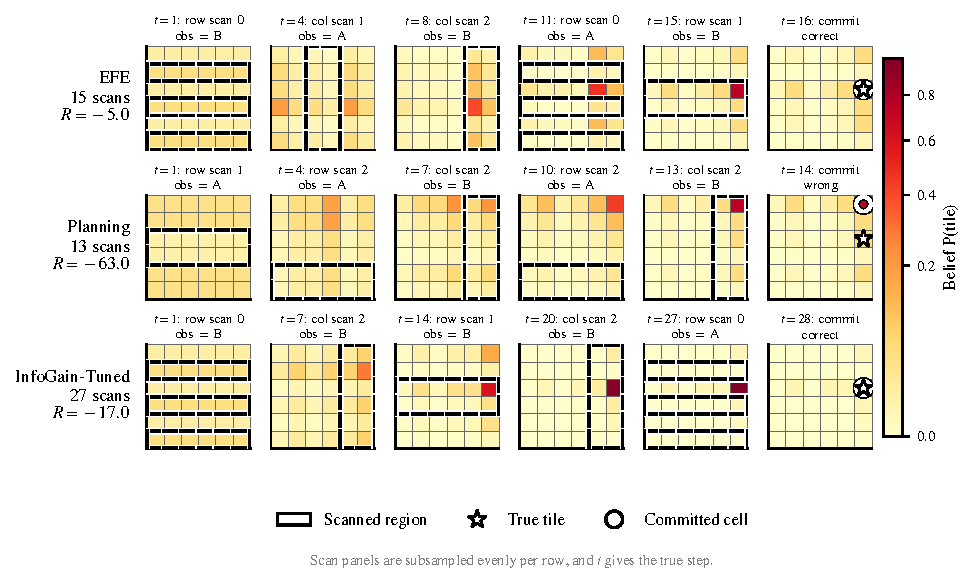
\includegraphics[width=\linewidth]{figures/fig_tileworld_comparison.pdf}
\caption{Agent comparison on the same $6{\times}6$ Tileworld episode. All agents start from the identical uniform prior, stated here rather than drawn once per row. Belief probability is encoded by the shared colorbar on a square-root color scale. Black outlines mark the cell group queried by each scan, each panel's title reports that scan's noisy binary readout as $\mathrm{obs}{=}\mathrm{A}$ or $\mathrm{obs}{=}\mathrm{B}$ naming which half of the queried group the signal favors, the black-edged white star marks the true tile, and the black-stroked white ring marks the committed cell. Scan panels are subsampled evenly within each row, so columns are not time-aligned across rows and each panel's $t$ gives the true step. EFE (top) commits correctly with efficient scanning. Planning (middle) commits on the wrong cell after 13 scans. InfoGain-Tuned (bottom) over-scans well past the point of diminishing returns.}
\label{fig:tw_comparison}
\Description{Three rows of six six-by-six grid heatmaps, one row per agent, with a shared vertical colorbar decoding belief probability on a square-root color scale and a legend identifying the overlay marks. Each row shows five evenly subsampled scan panels and a final commit panel, and row labels give the agent name, scan count, and total reward. Black contiguous outlines mark the scanned cell group, each scan panel's title also reports the noisy binary outcome of that scan as obs equals A or obs equals B, naming which half of the outlined group the scan's signal favors, a black-edged white star marks the true tile, and a black-stroked white ring marks the committed cell. In the top row belief concentrates into a single dark red cell and the EFE ring coincides with the star after 15 scans. In the middle row Planning commits after 13 scans on a cell two rows above the star in the same column, ending at reward minus 63. In the bottom row InfoGain-Tuned reaches a 0.98 belief on the correct cell but only after 27 scans.}
\end{figure}

\paragraph{Spatial scaling.} We scale the grid from $4{\times}4$ to $8{\times}8$ with five agents, Myopic, Planning, InfoGain-Tuned, Planning+IG, and EFE (Figure~\ref{fig:tw_scaling}). The sweep is a separate run from the full seven-agent Tileworld battery, of which Table~\ref{tab:tileworld} shows four rows, at the smaller episode count stated in the figure's caption, and it omits that battery's untuned Info Gain ($w{=}1$) and Epistemic-only agents. The full battery's per-agent tables, which exist at $6{\times}6$ and $8{\times}8$ and list all seven agents, are in Appendix~\ref{app:full_tables}. At $8{\times}8$ ($|S|{=}64$), reward-only Planning collapses to $1.4\% \pm 0.3$pp success while EFE maintains $69.4\% \pm 1.0$pp (seed-level SE). The mechanism behind that contrast matters, because the headline number is easy to over-read. At $8{\times}8$ reward-only Planning takes zero scans and is bit-identical to Myopic on every outcome metric ($0.00$ scans, $1.4\%$ success, $-49.16$ reward for both). A single binary scan of a $64$-cell belief cannot repay its cost within an $H{=}2$ lookahead. A depth-2 lookahead can see at most two scans before it must value a commit at its leaf, and after two binary scans a belief that began uniform over $64$ cells is still spread over many cells. The commit valued at that leaf therefore remains close to chance, and its expected improvement over committing at once is smaller than what the scans cost. Planning therefore never scans at all, and the comparison at this scale is really EFE against a non-scanning agent. This is a joint horizon-and-scale effect at the fixed $H{=}2$ of this sweep, not evidence about reward-only planning at deeper horizons, where the scan would begin to pay for itself.

Across scales, the gap between EFE and Planning is a threshold at $8{\times}8$ rather than a gradual widening. At $4{\times}4$ and $6{\times}6$, EFE's reward and success are within sampling error of reward-only Planning's, within 1 SE at both scales, with Planning nominally slightly ahead on both. No formal test was run for this specific sweep. EFE's advantage opens up only at $8{\times}8$, exactly where Planning's success collapses.

One further comparison in Figure~\ref{fig:tw_scaling} needs its own disclosure, because its two weighted series are not tuned the way the main tables' weighted agents are. Planning+IG at $w{=}100$ achieves $97.8\%$ success but at substantial reward cost due to extensive scanning. The scaling sweep fixes $w{=}100$ for both weighted agents, InfoGain-Tuned and Planning+IG, rather than tuning each separately as the main tables do, where the myopic Info Gain agent and the tree-search Planning+IG agent are each tuned within their own agent class. The figure is therefore a fixed-weight comparison and not a tuned one, and its InfoGain-Tuned series keeps that label from the main battery only as a series name.



\paragraph{Observation structure sensitivity.} A natural concern is whether EFE's advantage on Tileworld depends on the highly structured bit-level partition of scan actions. We test this by replacing the deterministic row/column splits with two alternative observation structures, random partitions and overlapping partitions. We run the test at the $6{\times}6$ scale of Table~\ref{tab:tileworld}. At that scale the advantage is the scan-count saving rather than a reward or success gap, so scan counts are the primary readout below, with reward and success reported alongside them. Under random partitions, each scan assigns the cells at random to two equal halves. The six splits therefore no longer correspond to separate index bits, and their answers are no longer guaranteed to combine into a unique cell, which is what the bitwise design's orthogonality provided. Under overlapping partitions, each scan draws a random weight for the row index and another for the column index, scores every cell by the weighted sum of its two normalized coordinates, and assigns the cell to one group or the other according to whether that score exceeds a random threshold. Each scan therefore splits the grid along a random tilted line, and different scans cut off overlapping regions, producing correlated and partially redundant observations (construction in \texttt{rho\_\allowbreak aif/\allowbreak environments/\allowbreak tileworld.py}).

The finding is that no partition mode separates EFE from Planning on reward or on success, while EFE uses fewer scans than Planning under all three. This battery is a separate run at 200 episodes per seed rather than the larger count of Table~\ref{tab:tileworld}, so its bitwise figures differ slightly from that table's. On $6{\times}6$ Tileworld ($H{=}2$, 200 episodes $\times$ 5 seeds, \texttt{results\_\allowbreak partition\_\allowbreak sensitivity\_\allowbreak 6x6.csv}, \texttt{experiments/\allowbreak run\_\allowbreak tileworld.py partition}), we report EFE against Planning in reward $\pm$ seed-level SE, with success in parentheses. Under the bitwise partition the pair is $-21.62 \pm 0.87$ (71.9\%) vs.\ $-21.41 \pm 0.64$ (73.6\%). Under the random partition it is $-29.31 \pm 0.43$ (56.1\%) vs.\ $-30.32 \pm 0.66$ (55.1\%). Under the overlapping partition it is $-47.53 \pm 0.73$ (8.5\%) vs.\ $-47.66 \pm 0.68$ (8.4\%). No partition mode separates the two agents on reward at the seed level, the largest gap being $1.01$ reward under the random partition at $1.28$ seed-level SE of the difference (Welch $p{=}0.24$). The nominal ordering itself changes direction across modes, with Planning nominally ahead under the bitwise partition and EFE nominally ahead under the random and overlapping ones. Planning is nominally ahead on success under the bitwise partition, but on success the two are within sampling error of each other under all three partition modes. On scans, where the main $6{\times}6$ result lives, EFE stays ahead of Planning under all three modes, meaning that it uses fewer scans ($14.76$ vs.\ $15.57$ bitwise, $12.97$ vs.\ $13.38$ random, $2.63$ vs.\ $2.70$ overlapping).

An earlier unseeded version of this experiment showed EFE nominally ahead of Planning on reward under the bitwise partition, and the seeded rerun reverses that reward ordering. That reversal is itself the clearest evidence that the nominal reward gaps here are sampling noise rather than signal. What the battery does establish is a large and consistent effect of observation structure on every agent. Both alternative modes cut absolute performance sharply, from roughly $-21$ reward under the bitwise partition to $-30$ under random scans and $-48$ under overlapping ones, because less complementary scans leave less recoverable information for any agent to exploit. We therefore treat the Tileworld result as scoped to the structured partition it was measured on, and we do not claim this experiment establishes EFE's advantage is model-independent.

\subsection{RockSample as an Interleaved Observe-Act Setting}
\label{app:rocksample_main_details}

To exercise Proposition~\ref{prop:factored}'s scope beyond observe-then-commit settings, we evaluate on a cost-modified variant of RockSample \citep{smith2004}, a widely used POMDP benchmark with interleaved observe-act dynamics (Section~\ref{sec:experiments} states the six deviations from the original). The agent moves on a grid among rocks of hidden quality, and the actions are the four cardinal moves (N/S/E/W), one check per rock, sample, and exit. Proposition~\ref{prop:factored} covers the check and navigation actions, and Remark~\ref{rem:transition-aware} states its boundary for state-altering sensing.

The agents under comparison fall into two groups. The first is the weighted family, meaning the Planning, Planning+IG, and EFE agents (Table~\ref{tab:rocksample} abbreviates Planning+IG as Plan+IG), which use depth-limited belief-space tree search over factored beliefs (independent per-rock). The search depth is the $d$ in each row label of Table~\ref{tab:rocksample}, depth 3 or 4 on the three smaller instances and depth 2 on RS[11,11]. All three share one hand-coded leaf evaluation (\texttt{rho\_\allowbreak aif/\allowbreak agents/\allowbreak rocksample\_\allowbreak agents.py}) that, at the depth limit, greedily plans the remainder of the episode. That leaf rule scores each rock not yet sampled by its belief-weighted sample value, the belief that the rock is good times the good-sample payoff plus the belief that it is bad times the bad-sample penalty. It considers only the rocks whose value is positive, moves to the one whose value net of the move cost of reaching it is highest and samples it, repeats, and exits when no such rock remains. Because these three agents share that leaf value, they differ only in the information gain weight $w$.

The second group holds the reference agents. POMCP is a genuine search-tree solver, run at a configuration tuned once on separate seeds and then held fixed (Appendix~\ref{app:rocksample}). The row labeled ``Rollout only'' runs POMCP's approach-then-check rule standalone, with no search tree. That rule is POMCP's rollout policy, the default policy that plays out each simulation once it leaves the search tree, and it is a hand-coded, unbounded-horizon rule rather than a depth-limited search. It walks to the unresolved rock with the highest belief per unit of distance (the nearest one at a uniform prior), checks it at close range where accuracy is $0.95$, samples if the belief crosses a threshold, writes off any rock whose belief falls below $0.15$, and exits when nothing is left. The prose below calls this standalone run the heuristic. Greedy, the remaining row, samples without checking.



Across the three smaller instances the reading is the same. EFE at $w{=}1$ is never significantly behind the $w{=}5$ comparator of Table~\ref{tab:rocksample}, is ahead of it once, and is statistically tied with or below the heuristic. On RS[5,3], EFE and Planning+IG ($w{=}5$) are not significantly different ($+16.47$ vs.\ $+16.41$, seed-level Welch $p{=}0.74$, a failure to reject, not a TOST-backed equivalence claim). Both are bolded in Table~\ref{tab:rocksample} as statistical ties with the best row, which is the heuristic at $+16.67$. On RS[7,4], EFE leads the weighted family outright ($+15.96$ vs.\ $+14.56$ for Planning+IG, $p<10^{-5}$) and is statistically tied with the heuristic's $+15.85$ ($p{=}0.65$, again a failure to reject rather than demonstrated equivalence). On RS[7,8], EFE and Planning+IG ($w{=}5$) are again not significantly different from each other ($+21.85$ vs.\ $+23.76$, $p{=}0.09$ uncorrected, not significant after Holm--Bonferroni), while both substantially outperform Planning ($+12.31$, $p<10^{-4}$). On this instance the heuristic reaches $+28.33 \pm 0.82$ on the identical protocol. Both deficits against it survive the per-metric Holm correction (Planning+IG $p{=}2.4{\times}10^{-3}$, EFE $p{=}4.6{\times}10^{-4}$), so the table bolds the heuristic alone there. Planning, Planning+IG, and EFE all sit below that $+28.33$, so on RS[7,8] these are relative comparisons within a family that is jointly suboptimal.

More checking beyond $w{=}5$ never significantly helps across these three instances, and twice significantly hurts. Planning+IG at $w{=}10$ (Appendix~\ref{app:rocksample}) falls to $+20.55$ on RS[7,8] ($p{=}0.003$, significant under the per-metric Holm family), so among the three nonzero weights we ran on RS[7,8], $w{=}5$ attains the highest reward. It is not significantly different from $w{=}1$. Raising Planning+IG's weight from $5$ to $10$ on RS[5,3] produces a decisive drop ($+14.60$ vs.\ $+16.41$, $p{=}3.5{\times}10^{-9}$). The same step from $5$ to $10$ on RS[7,4] is flat ($p{=}0.18$). On that instance EFE at $w{=}1$ had already beaten both tuned weights outright, so neither tuned weight is the one to beat there. We ran only $w \in \{5, 10\}$ as tuned comparators on RockSample, not the nine-point grid used for the observe-then-commit environments (Section~\ref{sec:methodology}), so this identifies the best of three sampled weights rather than a grid-searched argmax. We make no claim that $w{=}5$ is the reward-maximizing weight over a denser sweep.

The Bad column of Table~\ref{tab:rocksample}, the mean number of bad rocks sampled per episode, shows the information gain term at work, and the Good column beside it is the corresponding mean number of good rocks sampled. On RS[5,3], RS[7,4], and RS[7,8], EFE samples dramatically fewer bad rocks than Greedy, between $0.01$ and $0.06$ per episode (seed-level SE between $0.001$ and $0.013$) against Greedy's $1.51$ to $3.98$ (seed-level SE between $0.01$ and $0.05$), with seed-level Welch $p<5{\times}10^{-8}$ at every instance, confirming that the information gain term drives checking behavior.

EFE's gap over $w{=}0$ Planning, largest on RS[7,8] among the three smaller instances, does not extend to RS[11,11] ($|S|{=}2{,}048$), where EFE and Planning achieve identical reward ($+13.23$ each) despite that instance having the most rocks to check. Every tree-search agent vastly outperforms Greedy ($+12.9$ to $+13.2$ against $-18.9$), but nothing here differentiates EFE from reward-only planning. Every tree-search agent at its reported configuration converges to the same conservative pattern of checking one or two nearby rocks, sampling if a rock looks good, and exiting, so the weight on information gain moves reward by at most $0.06$. This includes POMCP at its frozen setting (Appendix~\ref{app:rocksample}). Moving from the table's depth 2 to depth 3 does not change this. Rerunning at depth 3 (\texttt{results\_\allowbreak rocksample\_\allowbreak 11x11\_\allowbreak depth3\_\allowbreak check.csv}) costs seconds and reproduces the same pattern within 1 SE, with Planning and EFE at $+13.23$ and Planning+IG at $+13.17$.

Two explanations fit that collapse. Either the instance leaves no exploitable slack, so every agent is already near the ceiling, or it leaves a great deal of slack that no depth-limited search can reach. The heuristic already in Table~\ref{tab:rocksample}, originally added for the POMCP comparison, settles which one holds, and the answer is not the flattering one. Recall that it is bound by no search depth and walks up to a rock before spending a check on it. Run on the same $5$ seeds and $100$ episodes as the table above, it scores $+28.66 \pm 0.83$ on RS[11,11], where every tree-search agent, EFE and POMCP included, sits in the $+12.94$ to $+13.23$ band. On RS[7,8] it scores $+28.33 \pm 0.82$ against the best tree-search agent's $+23.76 \pm 0.58$.

So the first explanation fails. There is a great deal of slack at 11 widely spaced rocks, and the depth-limited belief-space search cannot reach it. The Good column of Table~\ref{tab:rocksample} shows that slack in behavioral terms, since on RS[11,11] the heuristic samples $5.22$ good rocks per episode while every tree-search agent samples about half a rock.

The mechanism is now identifiable. Recall that check accuracy decays with the agent's distance from the rock (Section~\ref{sec:experiments}), so a check is informative only when taken from close range. Reaching close range means walking to the rock first. At this instance the checks that could be informative are far from the agent, and a depth-2 or depth-3 tree cannot represent the walk that would make them informative. Within its horizon only a single check taken from the agent's own starting cell is worth making, so the weight on information gain has almost nothing to act on. The shared greedy leaf rule values a rock at its belief-weighted sample reward, which is exactly zero at the uniform prior because at belief $0.5$ the $+10$ good-sample payoff and the $-10$ bad-sample penalty cancel. So no rock passes the rule's positive-value filter, and it recommends the exit. Because the informative checks lie beyond the depths we run, depth 3 leaves reward unchanged and every weight gives the same reward to within $0.06$, with the higher weights buying only about half an extra check per episode.

One further detail of that leaf deserves disclosure. Its completion estimate charges move costs for a walk to the east edge before collecting the exit reward (\texttt{rocksample\_\allowbreak agents.py}), while the environment pays the exit from any cell. This phantom travel cost deflates every depth-capped continuation relative to the exact value of exiting immediately, a bias toward earlier exits. The immediate exit escapes the deflation because an exit taken inside the tree at the current cell is valued at its true payoff, so only continuations that run on to the leaf carry the charge. Every agent in the family shares the phantom cost identically, so within-family comparisons are unaffected. But it means the leaf's exit recommendation is overdetermined here rather than resting on the zero prior expectation alone.

POMCP corroborates the mechanism from the other side. The heuristic profits from the far rocks because it walks up to each one before checking it, so that every check it spends is taken at close range where the check is accurate. A deeper POMCP tree gains the lookahead to plan a walk out to those rocks, but its in-tree check decisions are still taken from a distance, where accuracy is low. We read that from the behavioral trace in Appendix~\ref{app:rocksample} rather than deriving it from the search procedure. At the deepest horizon we ran, the tree spends many times more checks per episode than its own rollout policy does and still collects fewer good rocks. Given horizon enough to reach the distant checks, its reward falls monotonically, from $+12.94$ at $H{=}10$ to $-54.78$ at $H{=}40$, because the tours it assembles from noisy distant checks do not pay (Appendix~\ref{app:rocksample}). Both sides of the mechanism therefore point the same way. The heuristic walks up before checking and is bound by no depth, so it collects the slack. POMCP with a deeper horizon has the reach but still checks from a distance, so it does not. Reach alone, without walking up before checking, is not enough.

This is a limitation of the tree-search family at feasible depths on this instance, not evidence about information-gain weighting, and it bounds what RockSample[11,11] can be asked to show about EFE. Per-instance detail, including the Flat-MC reference (a flat one-ply Monte Carlo baseline with no search tree, kept in the appendix as a reference) and the standalone heuristic on every instance, is in Appendix~\ref{app:rocksample}.

The RS[11,11] collapse, the RS[7,8] advantage, and the Tileworld scaling result are one mechanism seen at three points rather than three unrelated per-instance results. EFE's advantage over reward-only Planning tracks how far the reward-only policy's default behavior already sits from the information-optimal one. On Tileworld, reward-only Planning scans too little to disambiguate a large grid, so directed information gain buys a large success-rate margin. On RS[7,8], eight rocks spread across a mid-sized grid leave real ambiguity about which are worth sampling, so choosing which rock to check pays off. On RS[11,11] the rocks sit far enough apart that no check beyond the agent's own cell is worth taking within the depths we run, so the weight has almost nothing to act on. The prediction this yields is that EFE's advantage should track how much slack a problem's structure leaves between the reward-only policy and the information-optimal one that the agent's search can actually represent, not problem size or observation-action count in themselves. We did not design or run instances specifically to stress-test that prediction, so it remains a mechanistic reading of the four RockSample instances and three Tileworld scales already reported rather than an independently validated scaling law.

\subsection{Structural Inspection}
\label{app:inspection_details}

To exercise Proposition~\ref{prop:factored}'s scope on a synthetic benchmark with an inspection structure and a larger state space than the environments above, we implement a Structural Inspection POMDP (Section~\ref{sec:experiments}). In that environment, the agent must declare each of the $N$ components nominal or faulty, a declaration that cannot be revised once made. A declaration is made while the agent stands on that component, and declarations are interleaved with the moves and tests. The instance names $N{=}8$ and $N{=}16$ below give the two instance sizes by their component count. Tests do not alter component states, so this is a factored observation POMDP and Proposition~\ref{prop:factored} applies. In Table~\ref{tab:inspection}, Missed is the mean number of faulty components per episode declared nominal, and Tests is the mean number of tests run per episode. As on RockSample, all tree-search agents here share one hand-coded leaf evaluation (\texttt{rho\_\allowbreak aif/\allowbreak agents/\allowbreak inspection\_\allowbreak agents.py}) that greedily completes the episode from the depth limit, so agents in this section differ only in the information-gain weight and not in their leaf value.



EFE ($w{=}1$) is a competitive untuned trade-off rather than uniquely best. On $N{=}8$ ($|S|{=}256$), Planning wins reward ($-17.85$), while EFE achieves $91.1\%$ accuracy ($-20.95 \pm 0.30$), gaining $+18.0$pp accuracy over Planning ($73.0\%$, seed-level Welch $p<10^{-10}$) at a moderate reward cost. Planning+IG ($w{=}5$) reaches $96.3\%$ accuracy but at $-27.98$ reward, over-testing relative to reward. On $N{=}16$ ($|S|{=}65{,}536$), Planning posts the best mean reward ($-45.42$), with EFE a close second at $-45.80$. EFE's deficit is not significant (seed-level $p{=}0.57$), so the two reward cells are bolded together. Planning+IG ($w{=}5$) wins accuracy ($97.3\%$) at substantial reward cost ($-54.74$, the worst of the three informed agents). That cost comes from extensive over-testing, $38.3 \pm 0.05$ tests vs.\ EFE's $28.1 \pm 0.09$ (seed-level SE), roughly $36\%$ more (seed-level Welch $p{=}1.7{\times}10^{-11}$). EFE outperforms Planning by $+12.6$pp accuracy ($90.8\%$ vs.\ $78.2\%$, seed-level $p<10^{-7}$) at a reward cost of only $0.39$ that is itself not significant, a far better accuracy-per-reward trade than Planning+IG's. The $N{=}16$ instance is the largest state space in our evaluation and shows that the factored belief tree search remains feasible at that size on this synthetic benchmark, with a known model and a hand-coded leaf rule. Validation on a deployed inspection problem is future work.

Inspection's payoffs also let us read off what Proposition~\ref{prop:nearopt} predicts about $w{=}1$ here, that is, whether $w{=}1$ falls inside its near-optimality interval. The reading is possible because the proposition's thresholds depend on the reward asymmetry ratio $\alpha = |R^-|/R^+$ (not the reward scale that Section~\ref{sec:collapse} also writes as $\alpha$), along with the observation accuracy and cost. The penalty structure is asymmetric on the missed-fault side. Declaring nominal pays $+2$ when correct and $-50$ when a fault is missed ($\alpha = 25$ for that decision, the missed-fault penalty divided by the correct-nominal reward), while declaring a fault is symmetric ($+5$ when correct, $-5$ on a false alarm, $\alpha = 1$). Reading Proposition~\ref{prop:nearopt}'s two-state thresholds onto this multi-state environment is a heuristic reduction, as with the two-state-reduced rows of Table~\ref{tab:alpha_eta}. With that caveat in place, the missed-fault decision, where the large penalty sits, places the environment in the proposition's large-asymmetry regime. In that regime Part (a) says that a heavy penalty for a wrong commit drives the lower threshold $w_{\mathrm{thresh}}$ downward (the proposition's $w^*_{\mathrm{thresh}}$, written without the star from Corollary~\ref{cor:pi4} onward), and once that threshold falls below zero, $w{=}1$ clears the interval's lower endpoint. The interval's upper endpoint, the over-observation threshold of Part (b), would then also have to exceed $1$ for $w{=}1$ to lie inside the interval, and we do not evaluate that threshold for Inspection. The reading is therefore that Inspection sits in the regime where Part (a) stops binding, which is the regime where the proposition predicts $w{=}1$ is a reasonable untuned default, and not a computed placement of $w{=}1$ inside the full interval.
